\section{Результаты работы программы}

В данном разделе представлены результаты выполнения всех пунктов заданий
лабораторных работ~1--5. Для каждого пункта приведён краткий обзор вывода
программного комплекса и соответствующая визуализация.

% ─────────────────────────────────────────────────────────────────
\subsection{Лабораторная работа~1}
% ─────────────────────────────────────────────────────────────────

\subsubsection{Генерация графа по распределению Рэлея--Райса}

Генерируется связный ациклический неориентированный граф. Пользователь
вводит число вершин~$n$ и параметры распределения~$a$ и~$h$. Число рёбер
и их распределение по степеням вершин определяются автоматически через
softmax-нормировку выборок из распределения Рэлея--Райса. Веса рёбер
генерируются по тому же закону.

Визуальное подтверждение корректности генерации весов представлено на
рис.~\ref{fig:graph_gen}: гистограмма сгенерированных значений с
наложенной теоретической плотностью вероятности $f(z; a, h)$.

\begin{figure}[H]
    \centering
    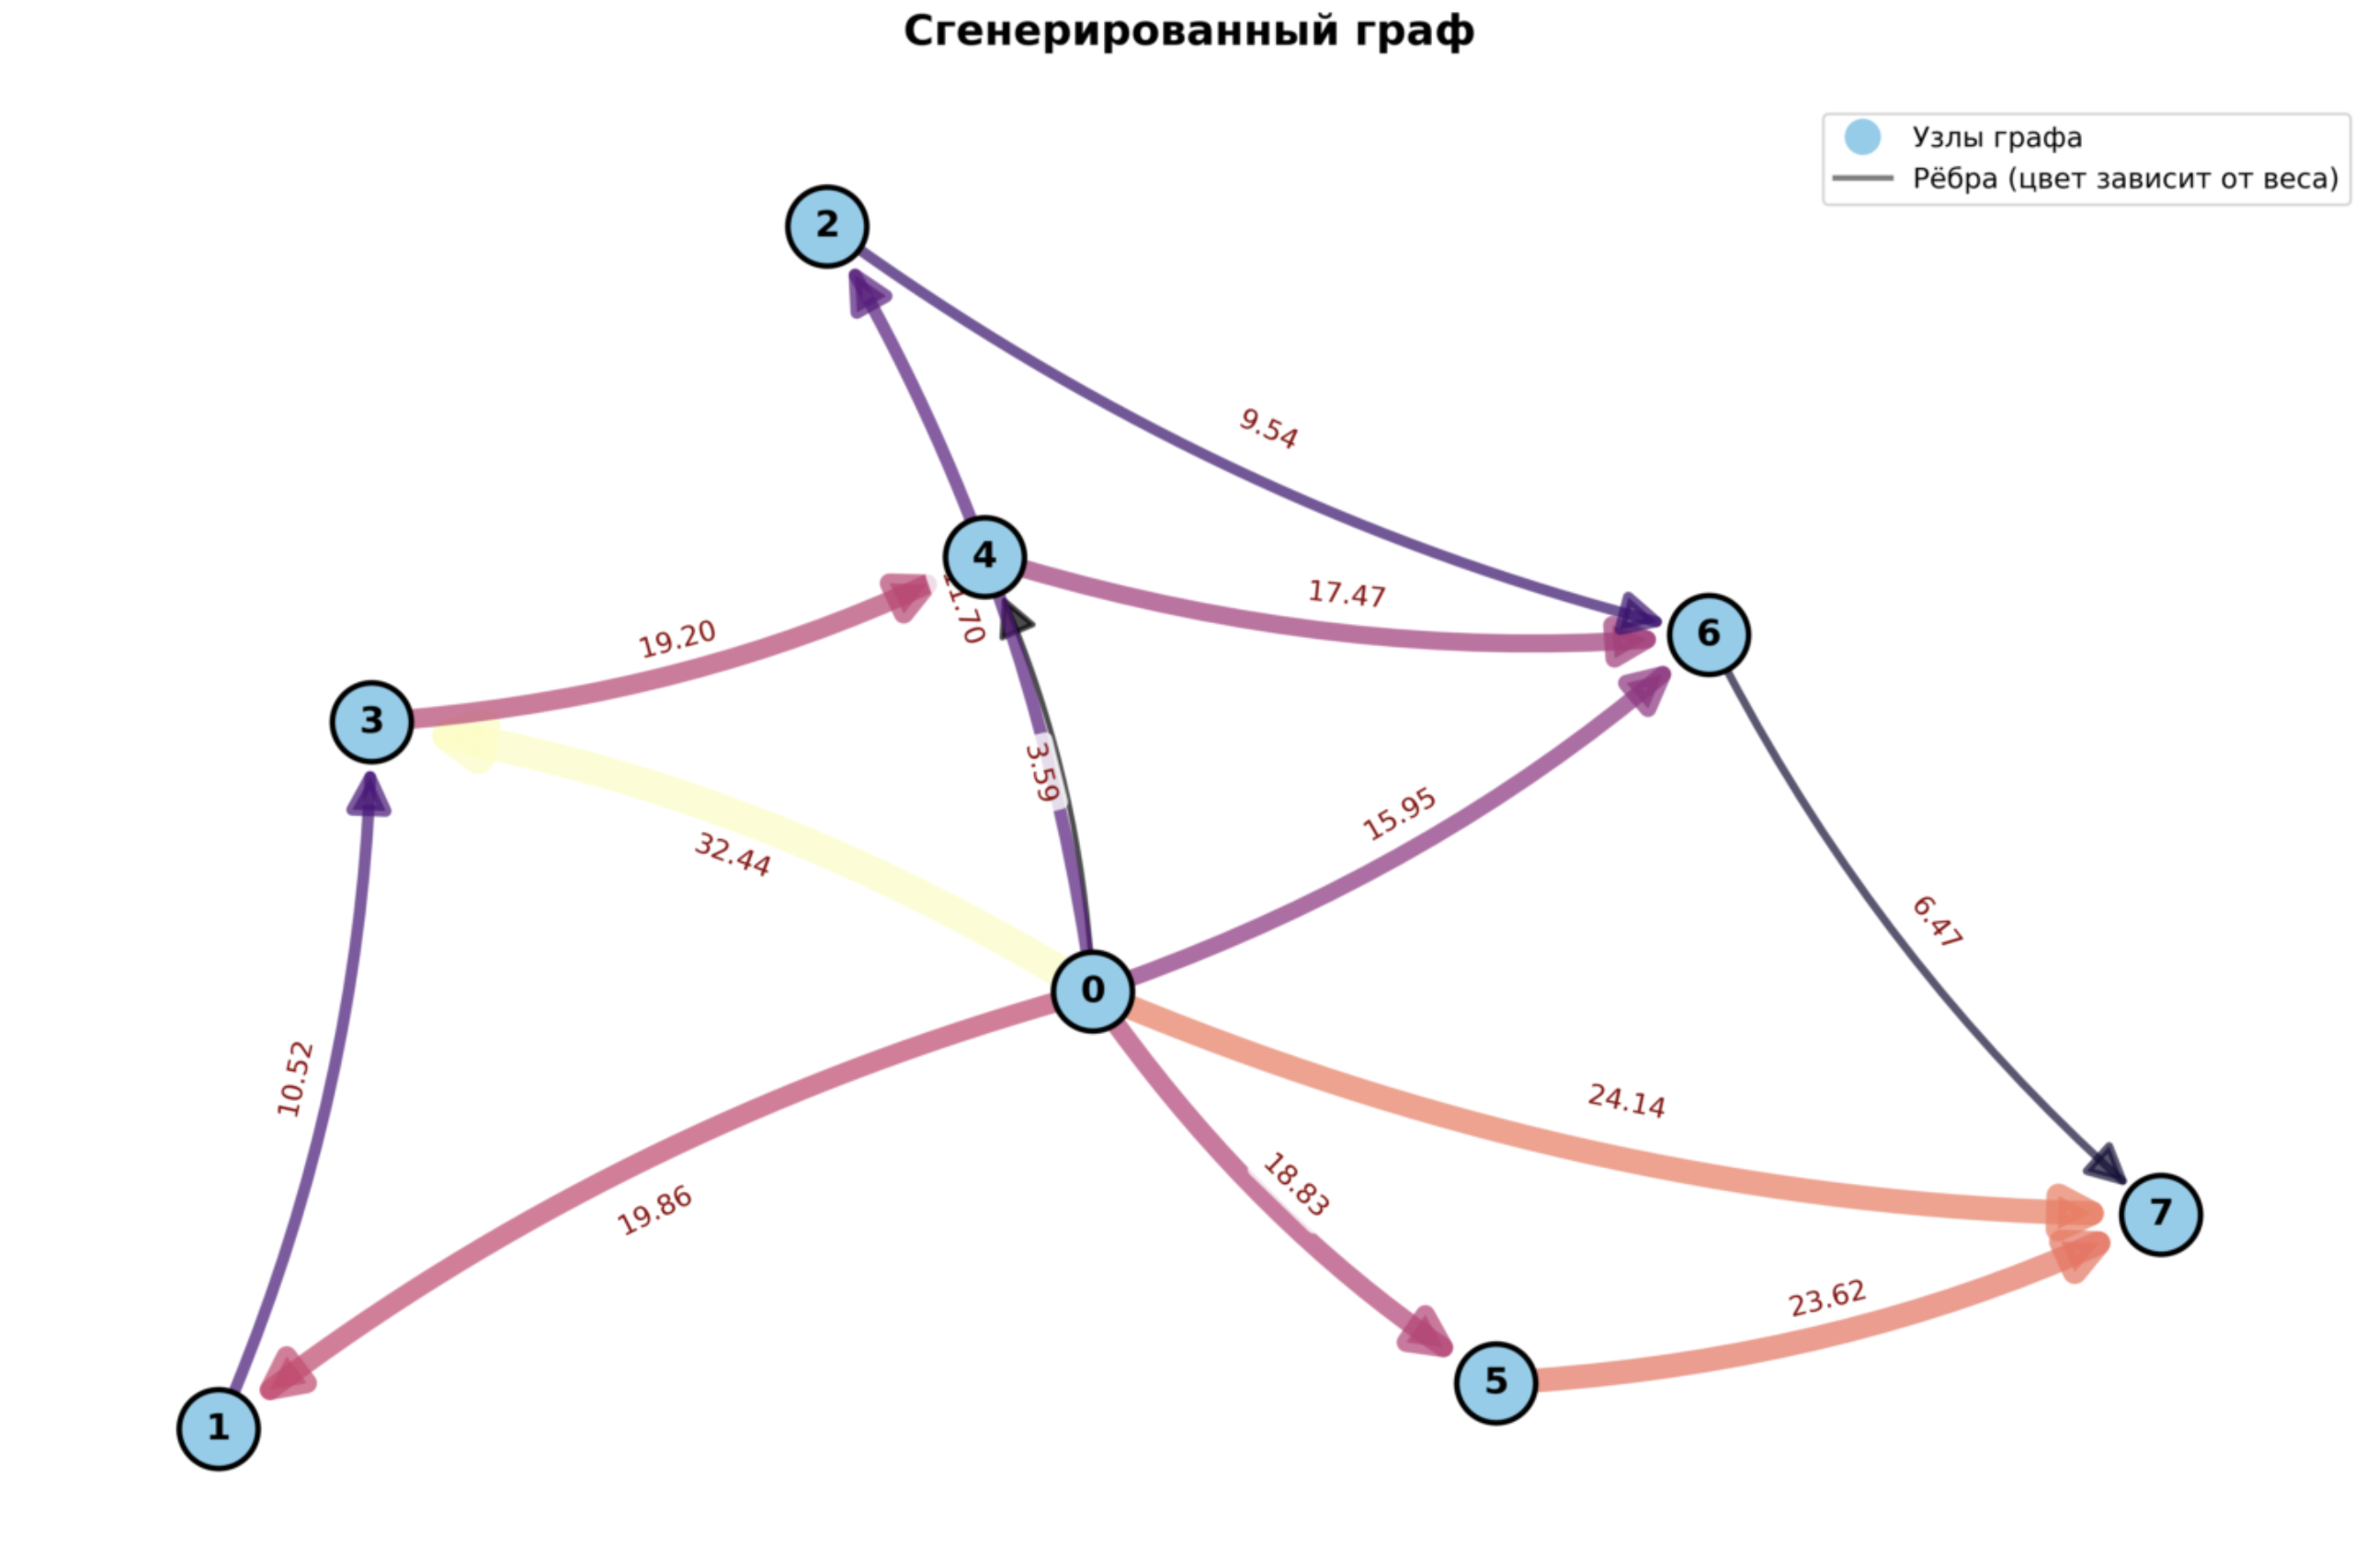
\includegraphics[width=0.7\linewidth]{images/lab1/graph.png}
    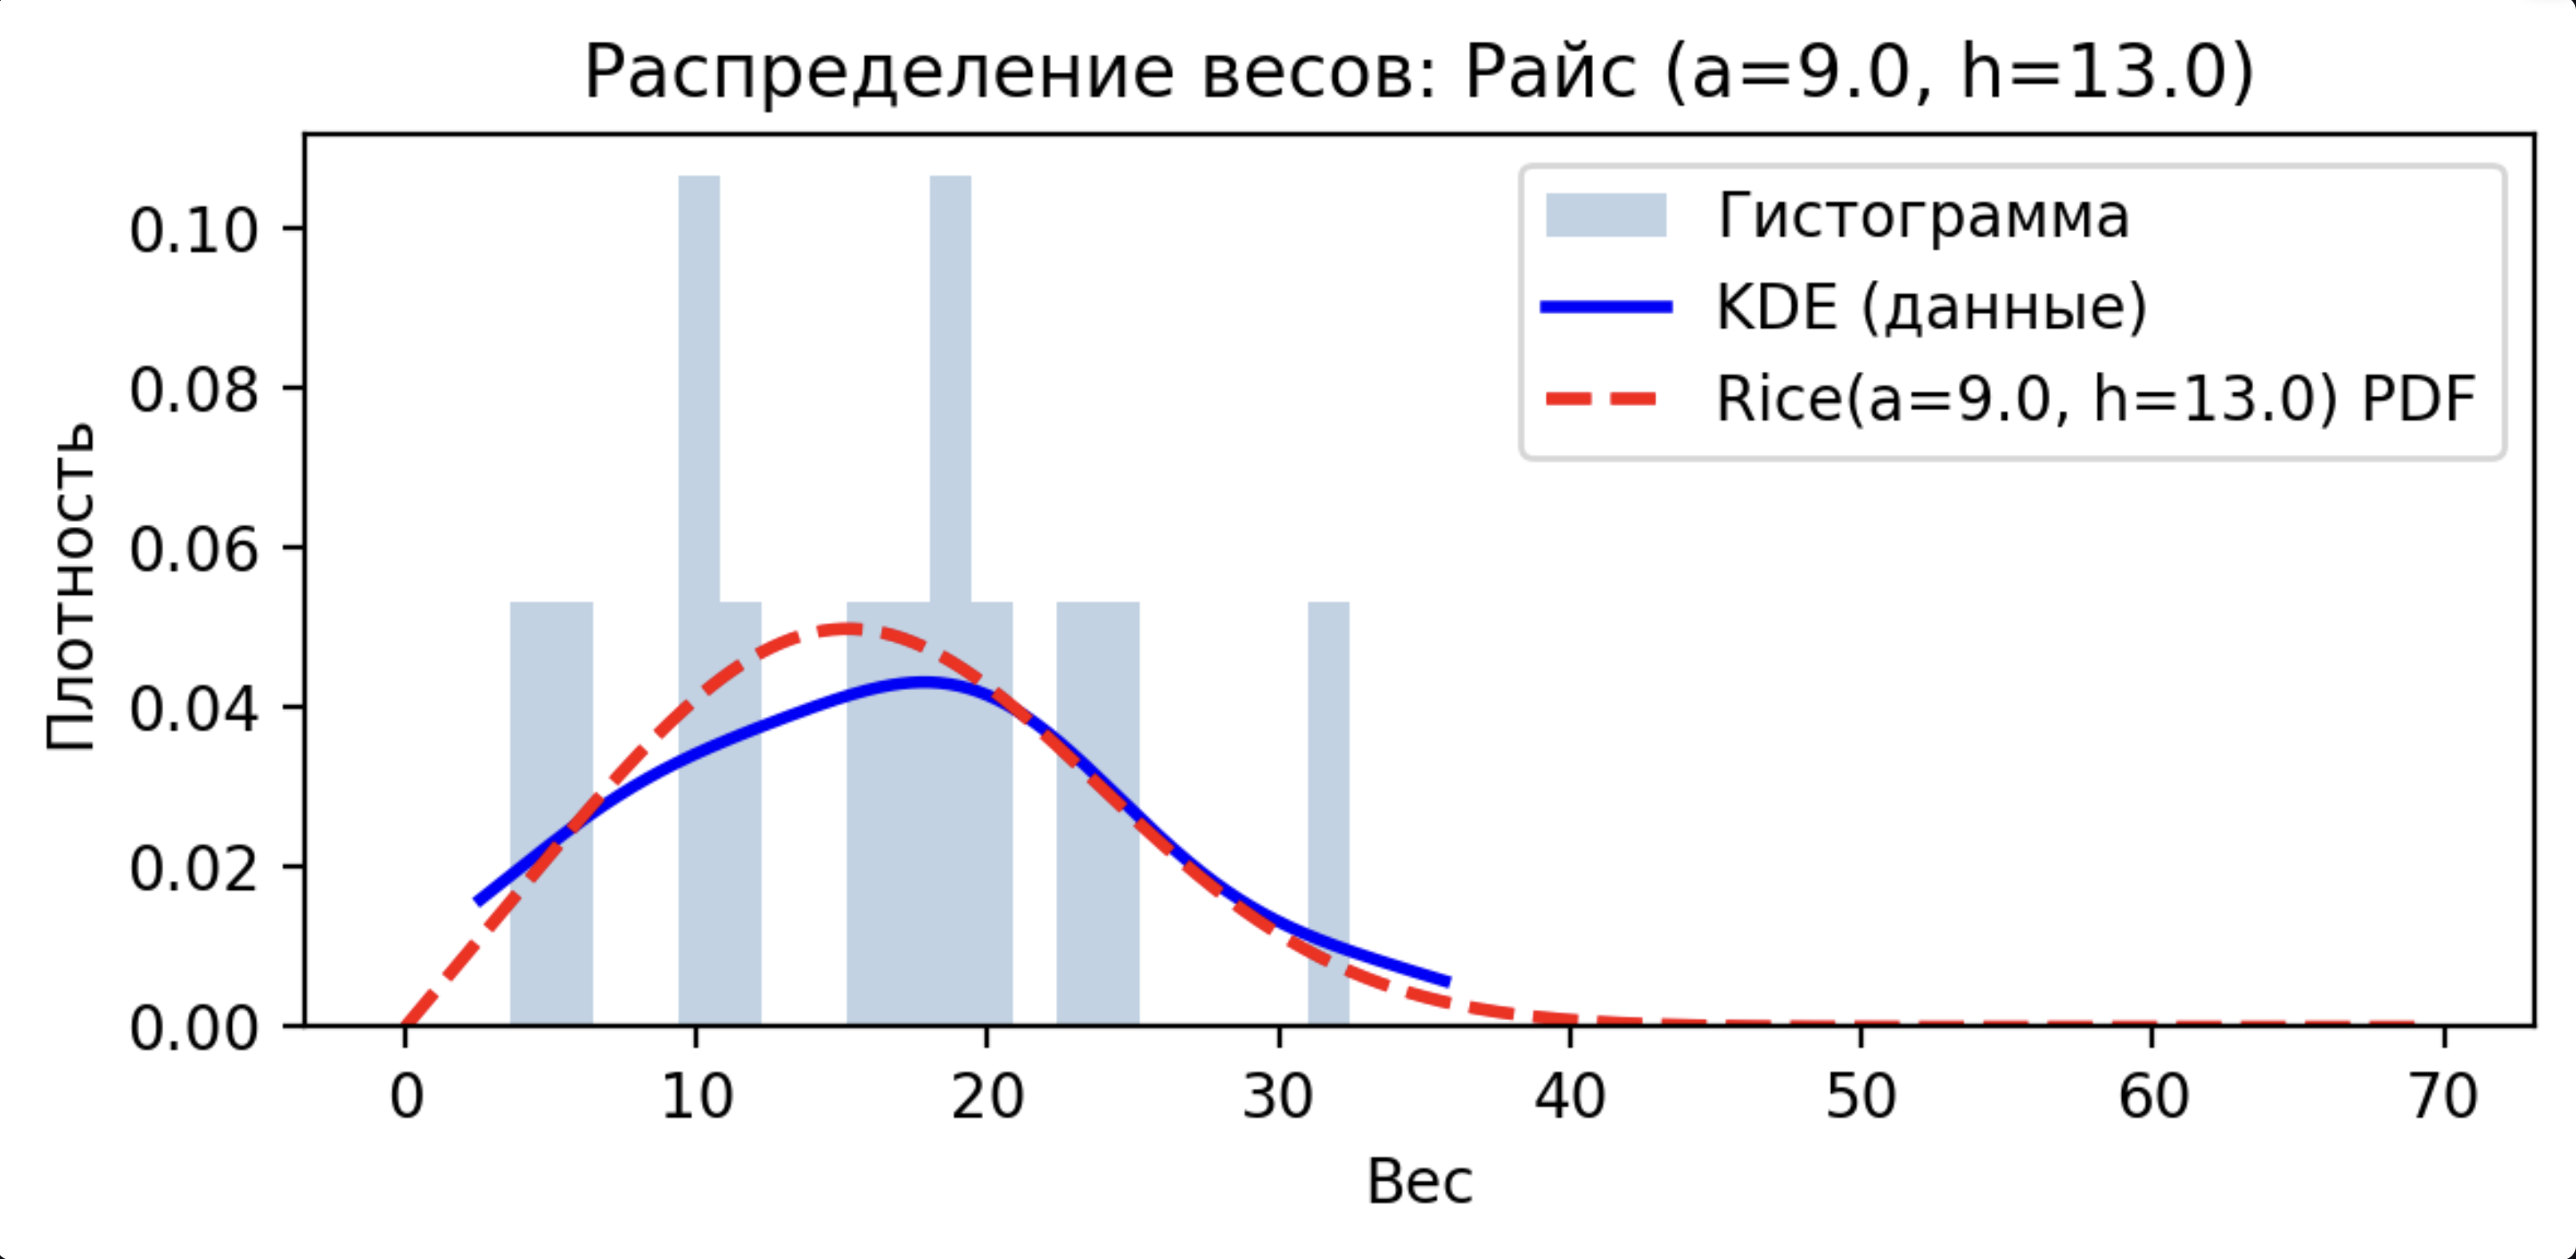
\includegraphics[width=0.7\linewidth]{images/lab1/dist.png}
    \caption{Сгенерированный граф и распределение весов рёбер}
    \label{fig:graph_gen}
\end{figure}

\subsubsection{Матрицы смежности и весов}

Программа экспортирует матрицу смежности и матрицу весов.
Результат приведён на рис.~\ref{fig:matrices_adj_weight}.

\begin{figure}[H]
    \centering
    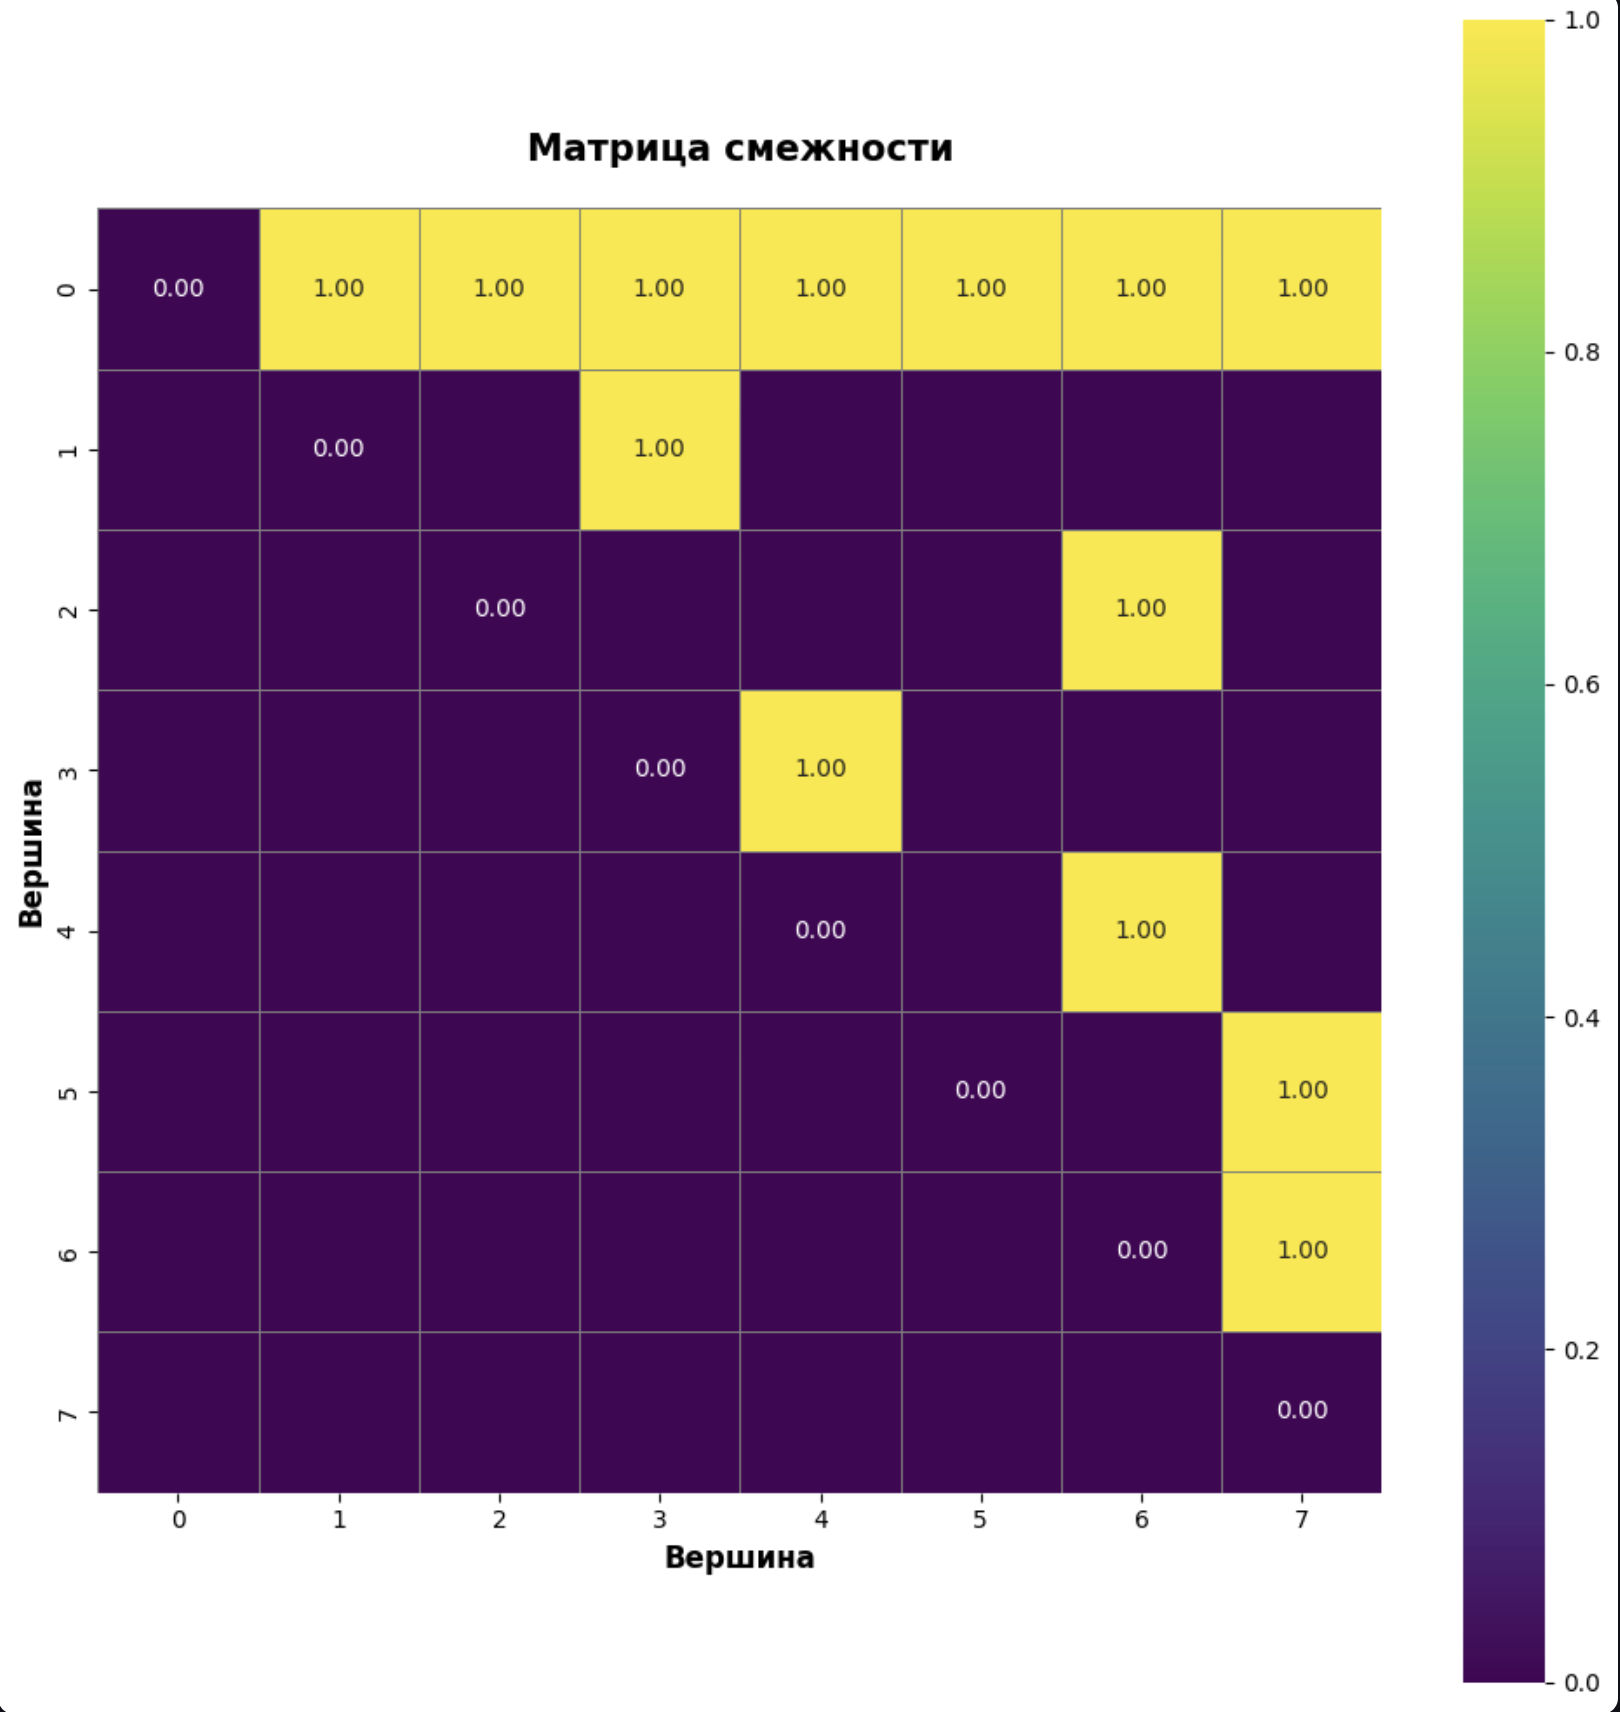
\includegraphics[width=0.48\linewidth]{images/lab1/adjency.png}%
    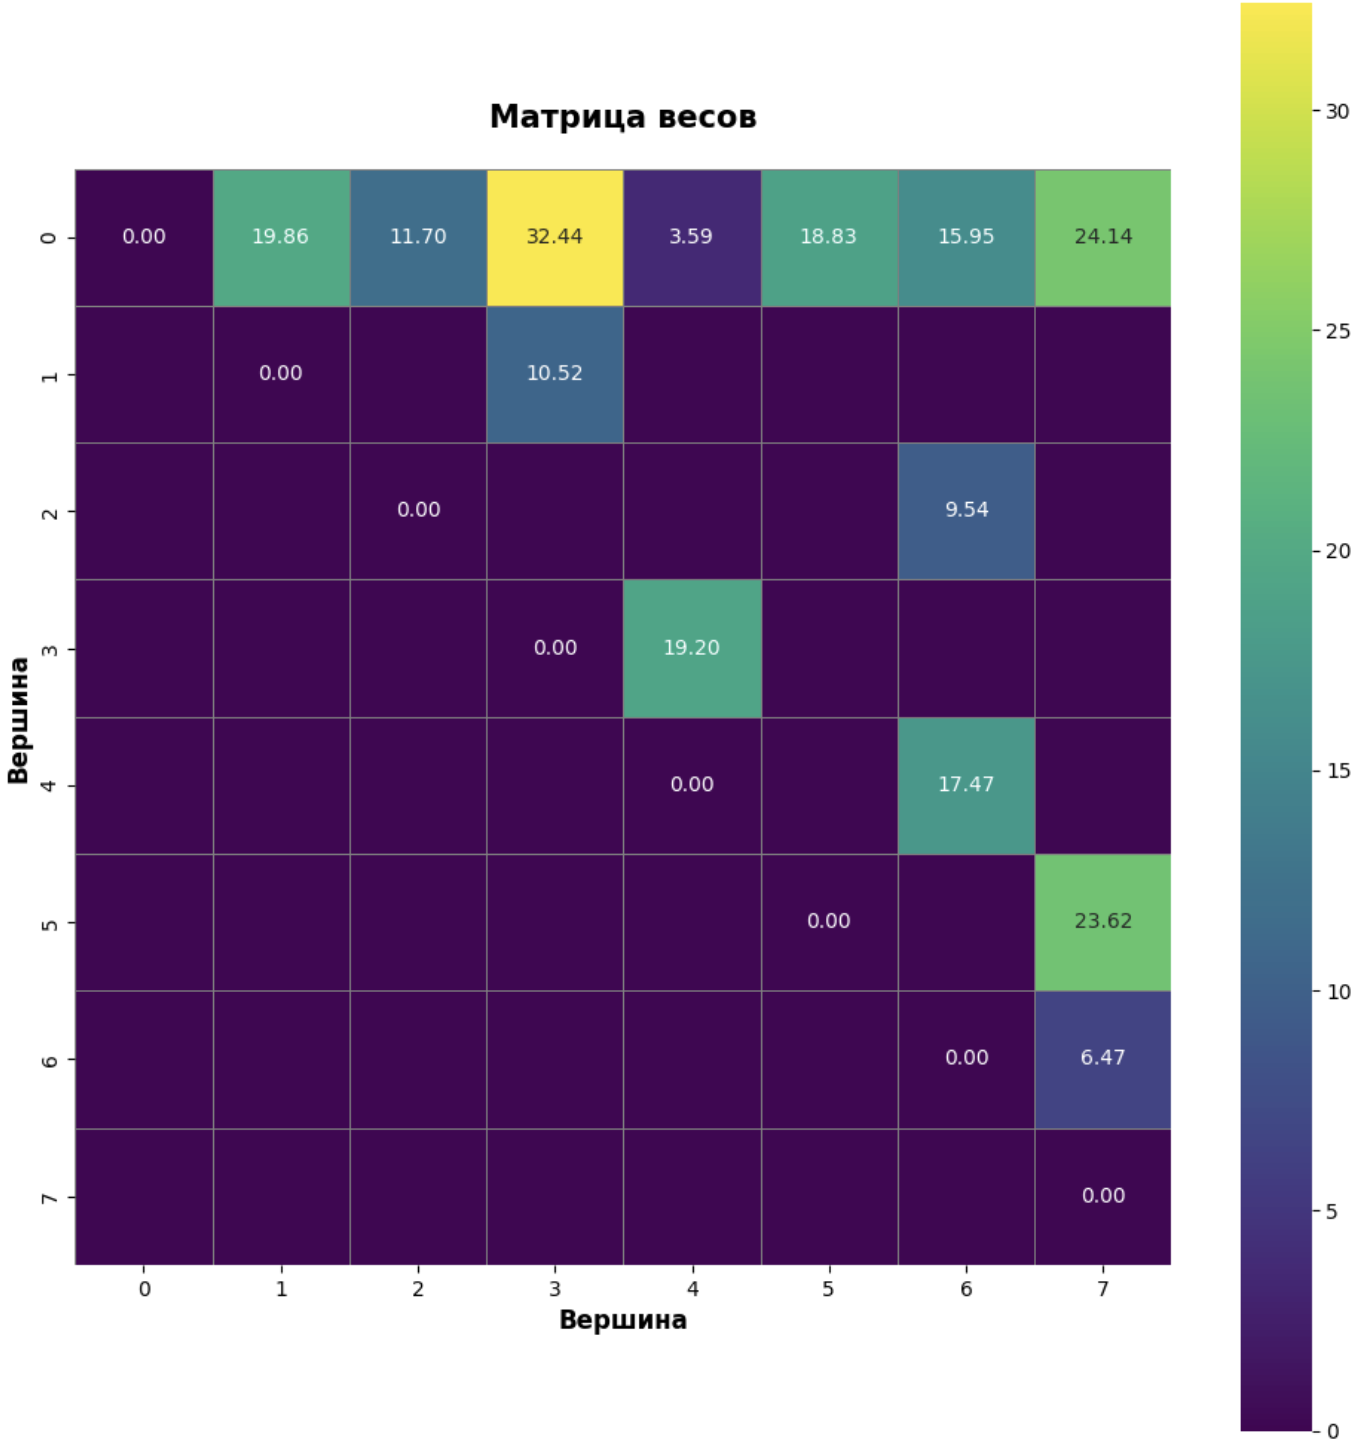
\includegraphics[width=0.48\linewidth]{images/lab1/weights.png}
    \caption{Матрица смежности (слева) и матрица весов (справа)}
    \label{fig:matrices_adj_weight}
\end{figure}

\subsubsection{Метод Шимбелла}

Программа строит две матрицы: минимальных и максимальных суммарных
весов маршрутов длины ровно~$k$. Матрицы для $k = V - 1$ показаны на
рис.~\ref{fig:shimbell}.

\begin{figure}[H]
    \centering
    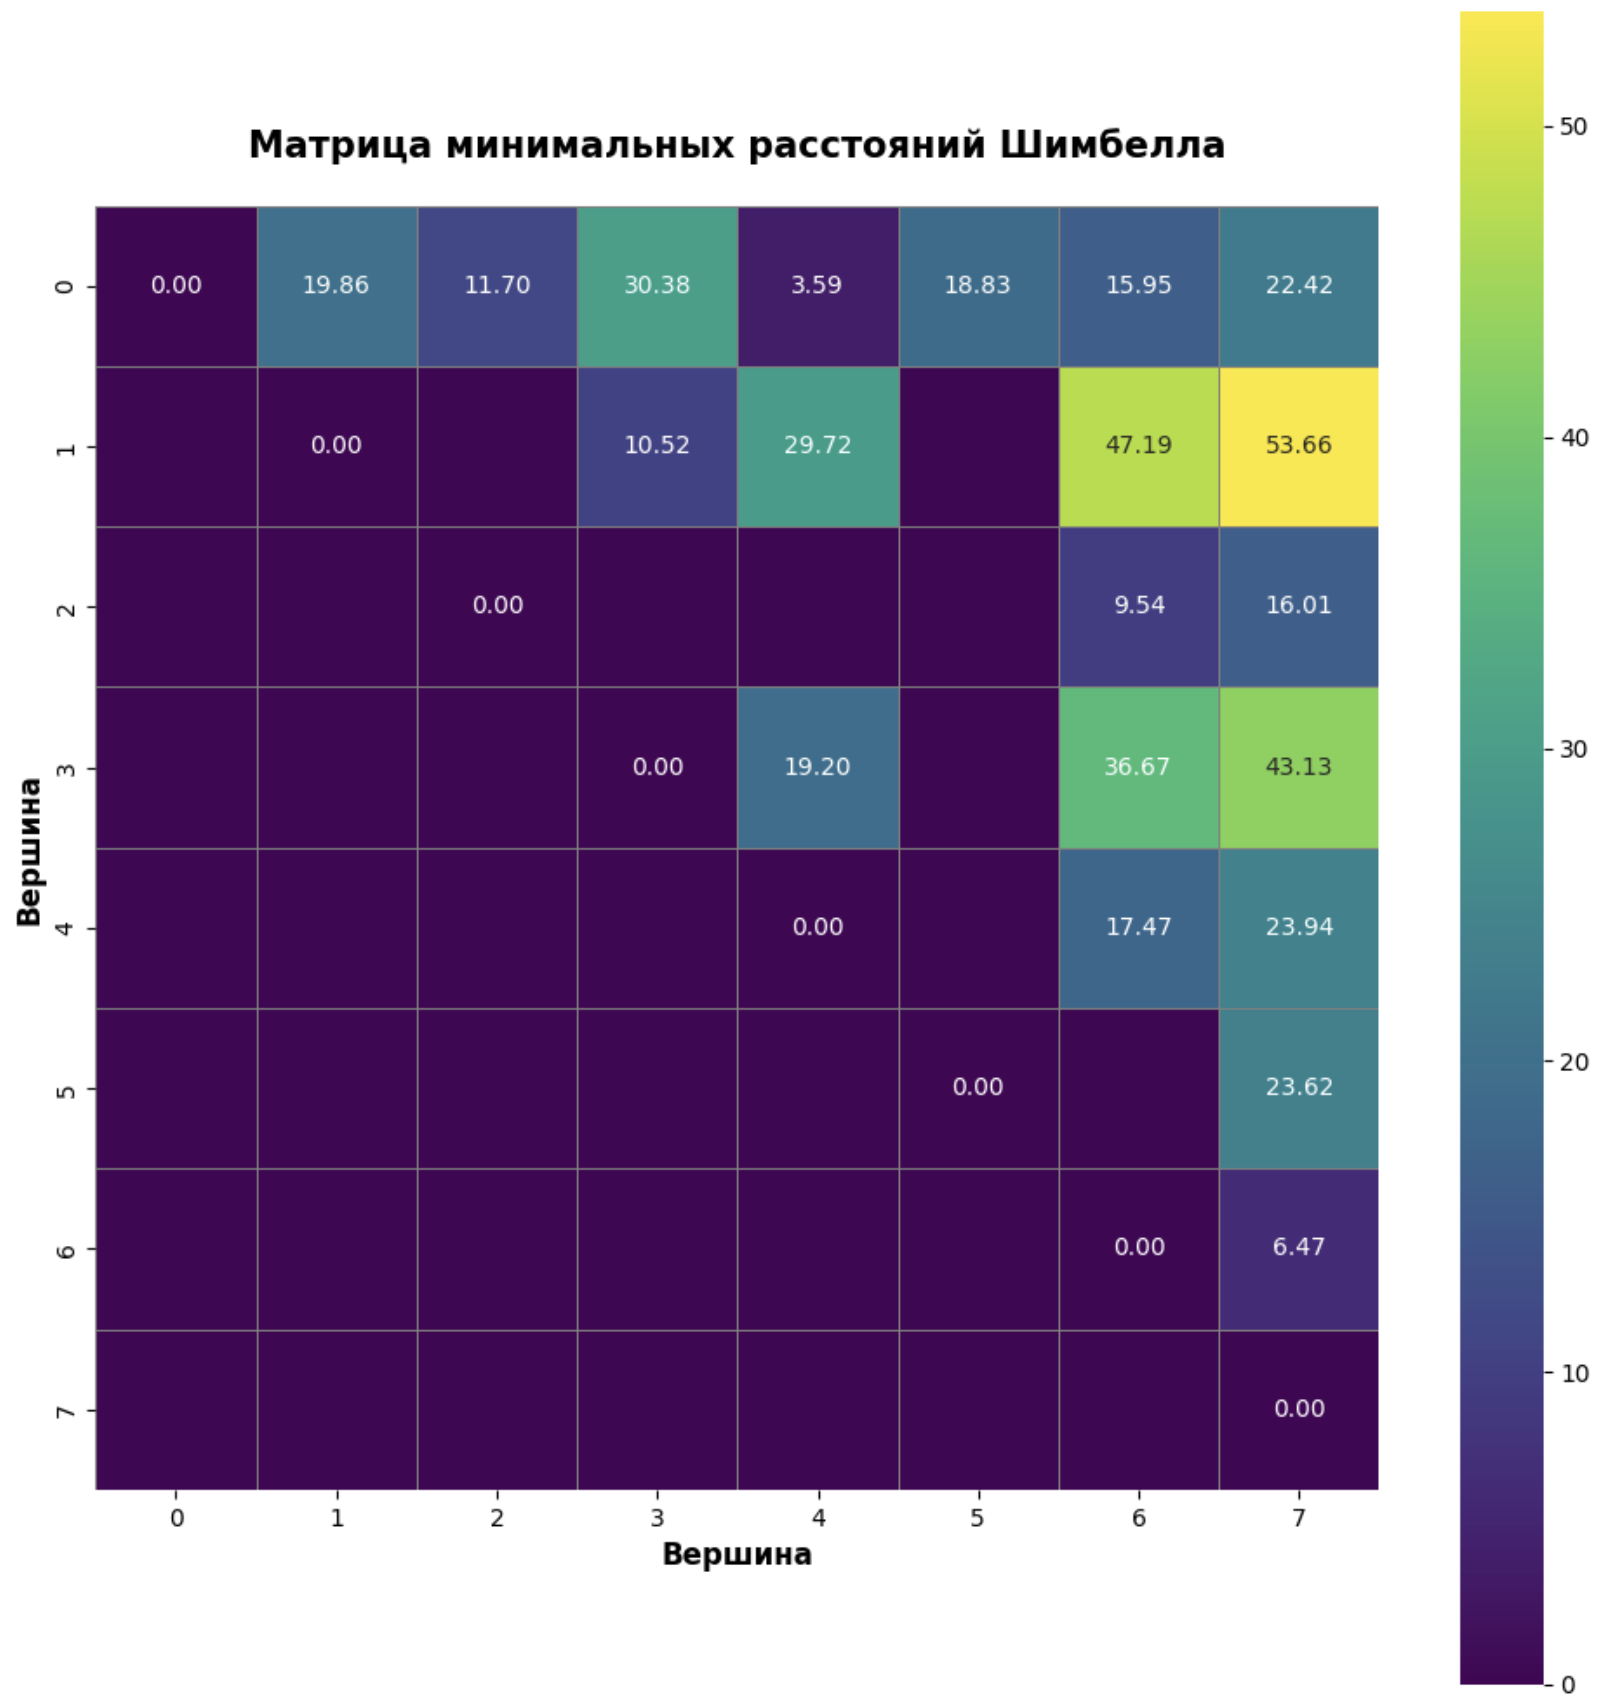
\includegraphics[width=0.48\linewidth]{images/lab1/minshimbell.png}%
    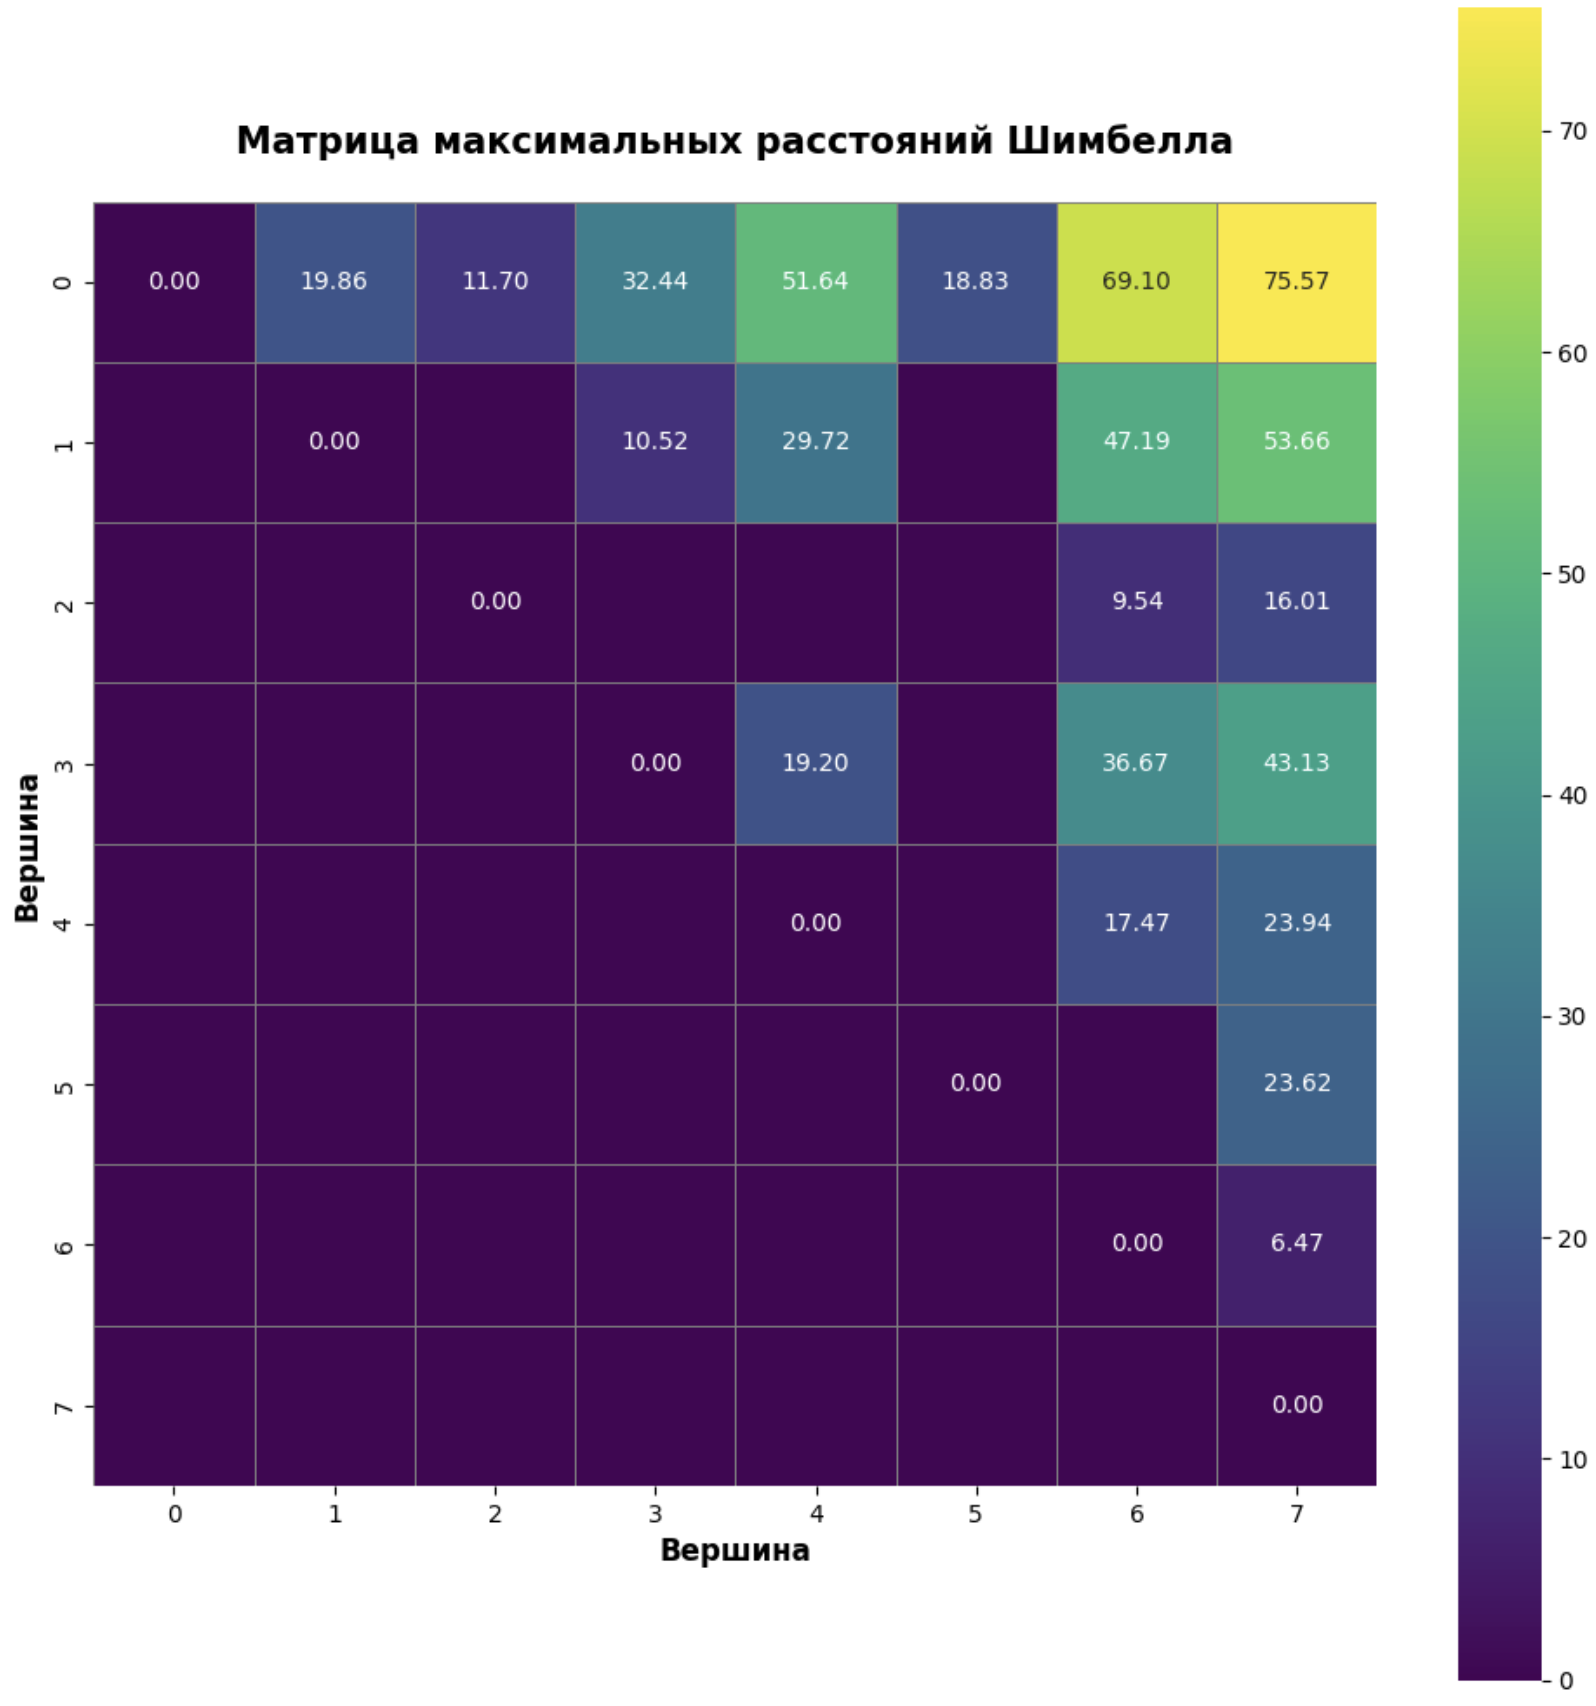
\includegraphics[width=0.48\linewidth]{images/lab1/maxshimbell.png}
    \caption{Матрицы Шимбелла для $k = V - 1$: мин (слева) и макс (справа) пути}
    \label{fig:shimbell}
\end{figure}

\subsubsection{Подсчёт всех маршрутов}

Пользователь вводит вершину-источник и вершину-цель. Программа находит
все простые пути методом поиска с возвратом и выводит их список в консоль.
На визуализации (рис.~\ref{fig:all_paths}) каждый путь выделен своим
цветом, рёбра остального графа отображаются серым.

\begin{figure}[H]
    \centering
    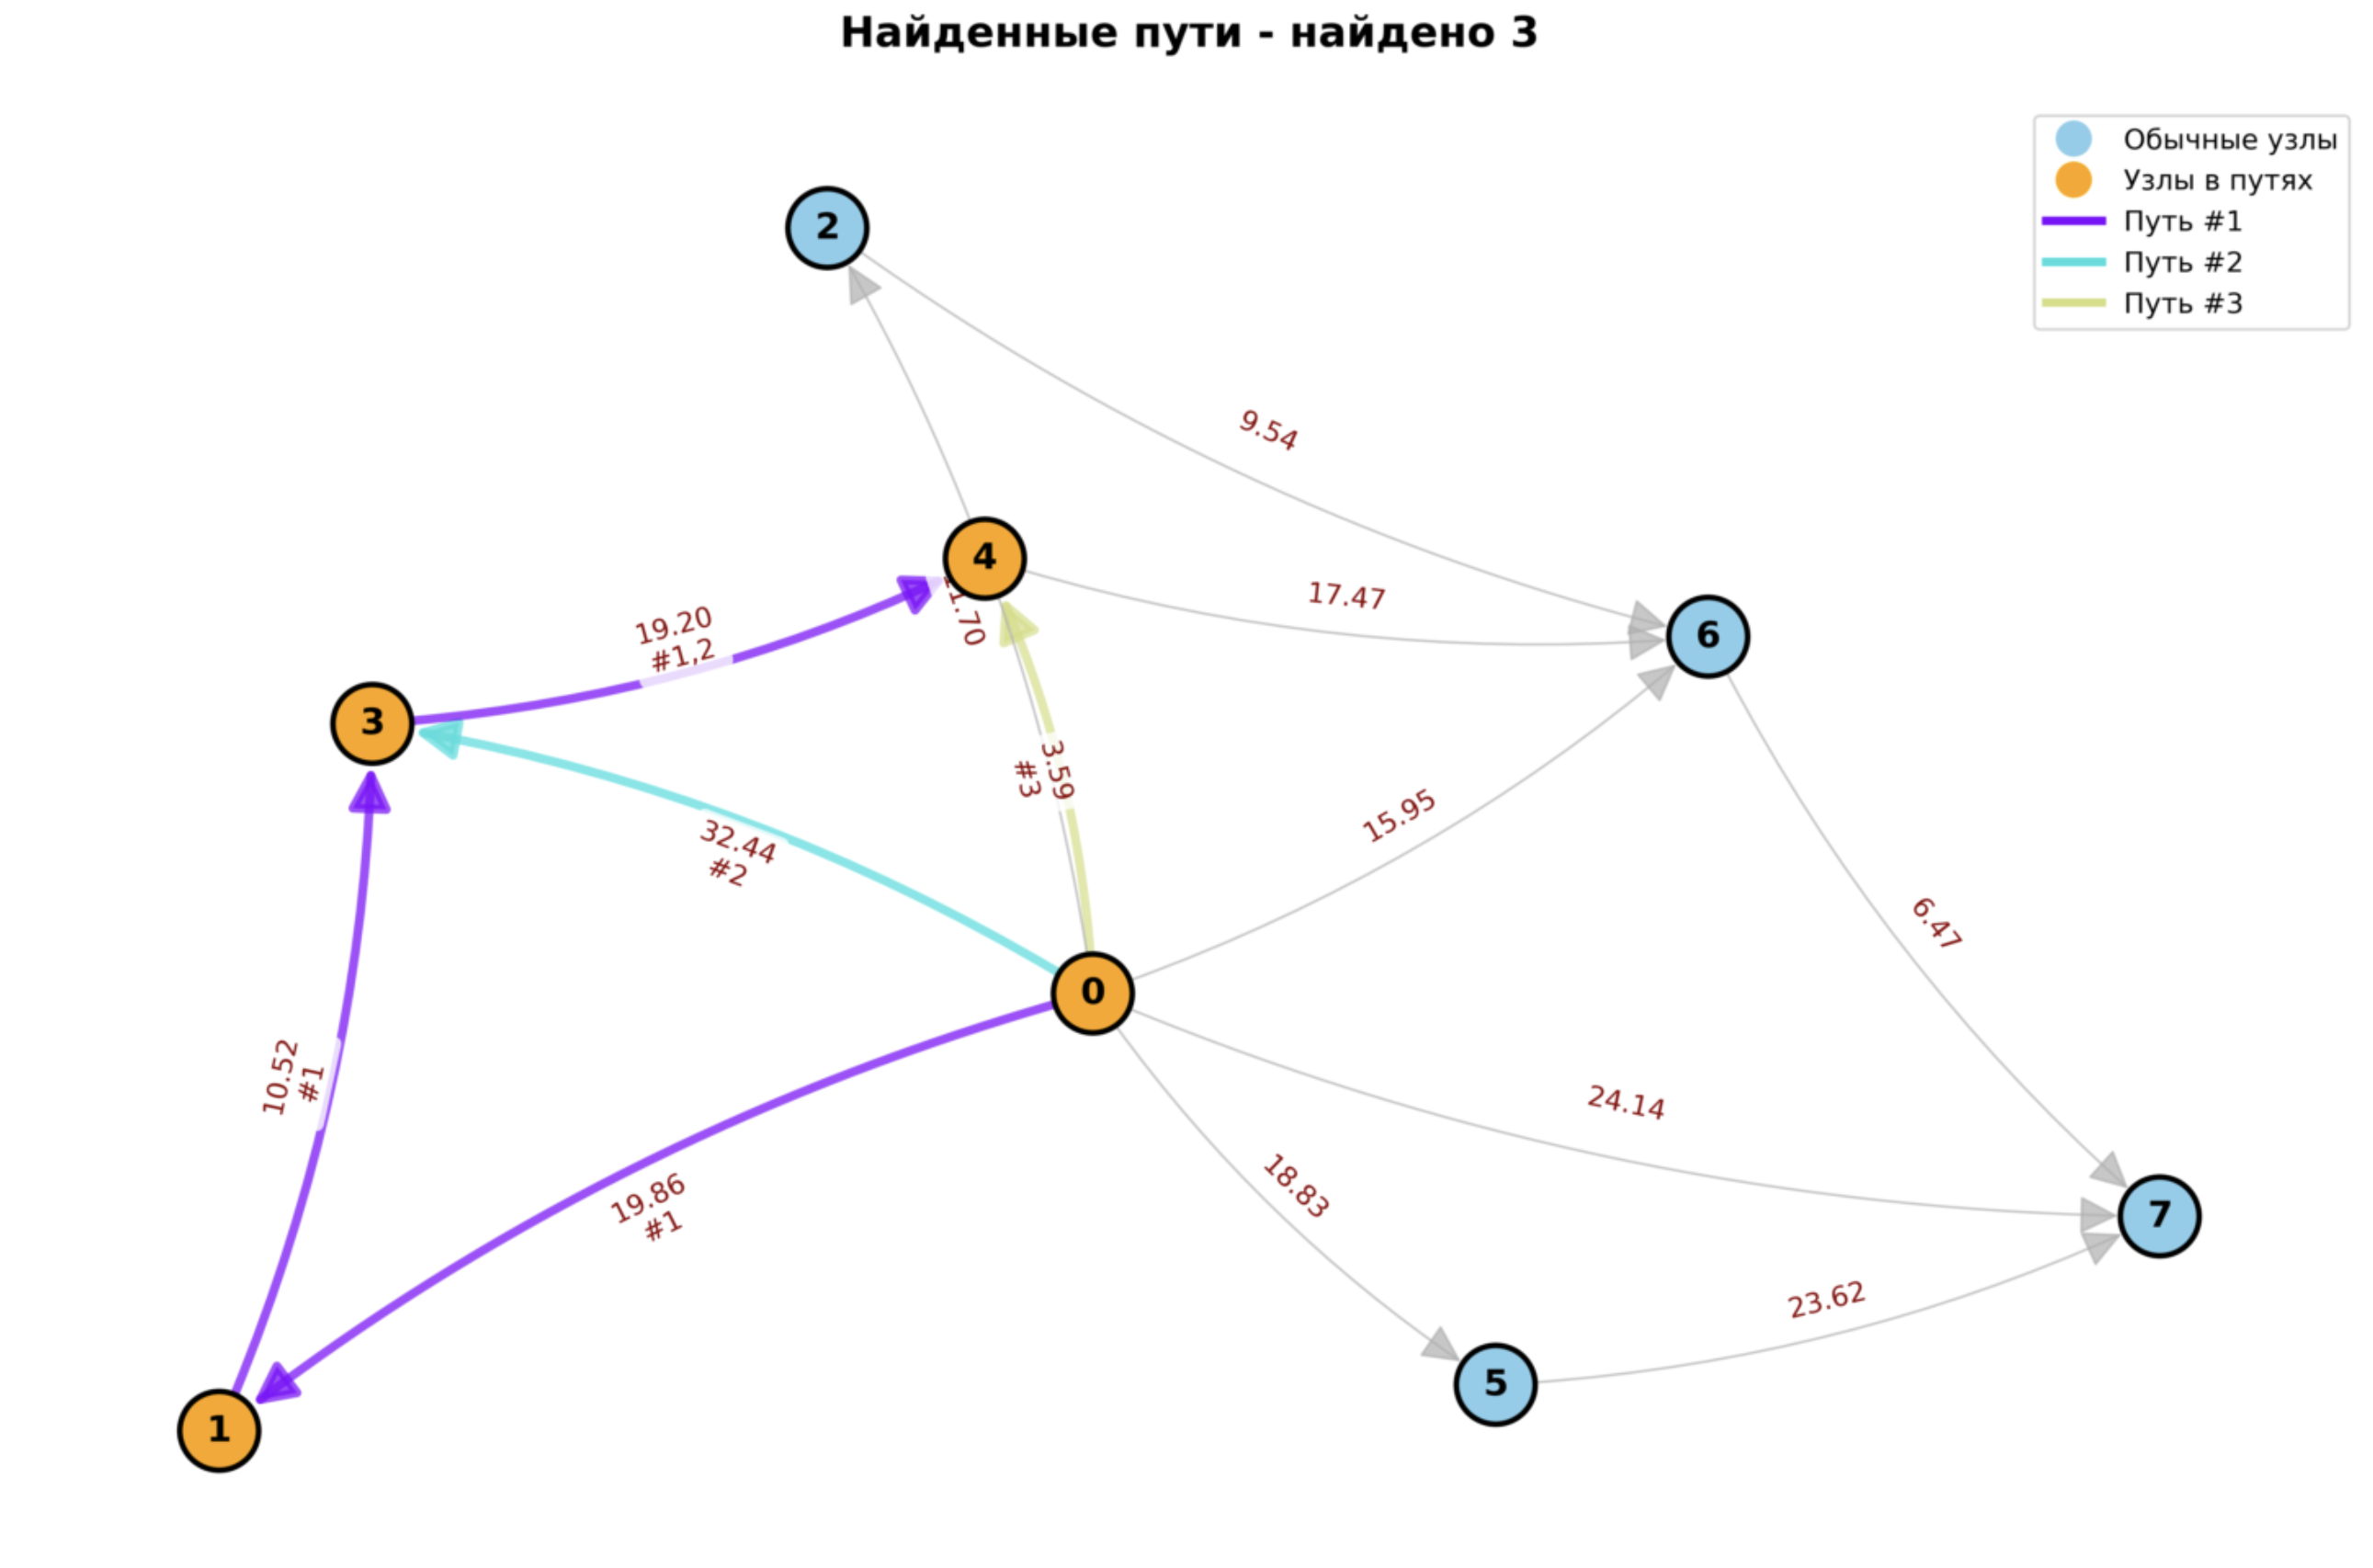
\includegraphics[width=1\linewidth]{images/lab1/paths.png}
    \caption{Все простые маршруты между заданными вершинами}
    \label{fig:all_paths}
\end{figure}

\subsubsection{Метрики графа: эксцентриситеты, центр, диаметр}

Программа вычисляет эксцентриситет каждой вершины через BFS, находит
радиус, диаметр, центральные и диаметральные вершины. На визуализациях
(рис.~\ref{fig:ecc_graph},~\ref{fig:ecc_diameter}) вершины раскрашены
по роли: центральные~--- одним цветом, диаметральные~--- другим.
Текстовый вывод приведён на рис.~\ref{fig:ecc_text}.

\begin{figure}[H]
    \centering
    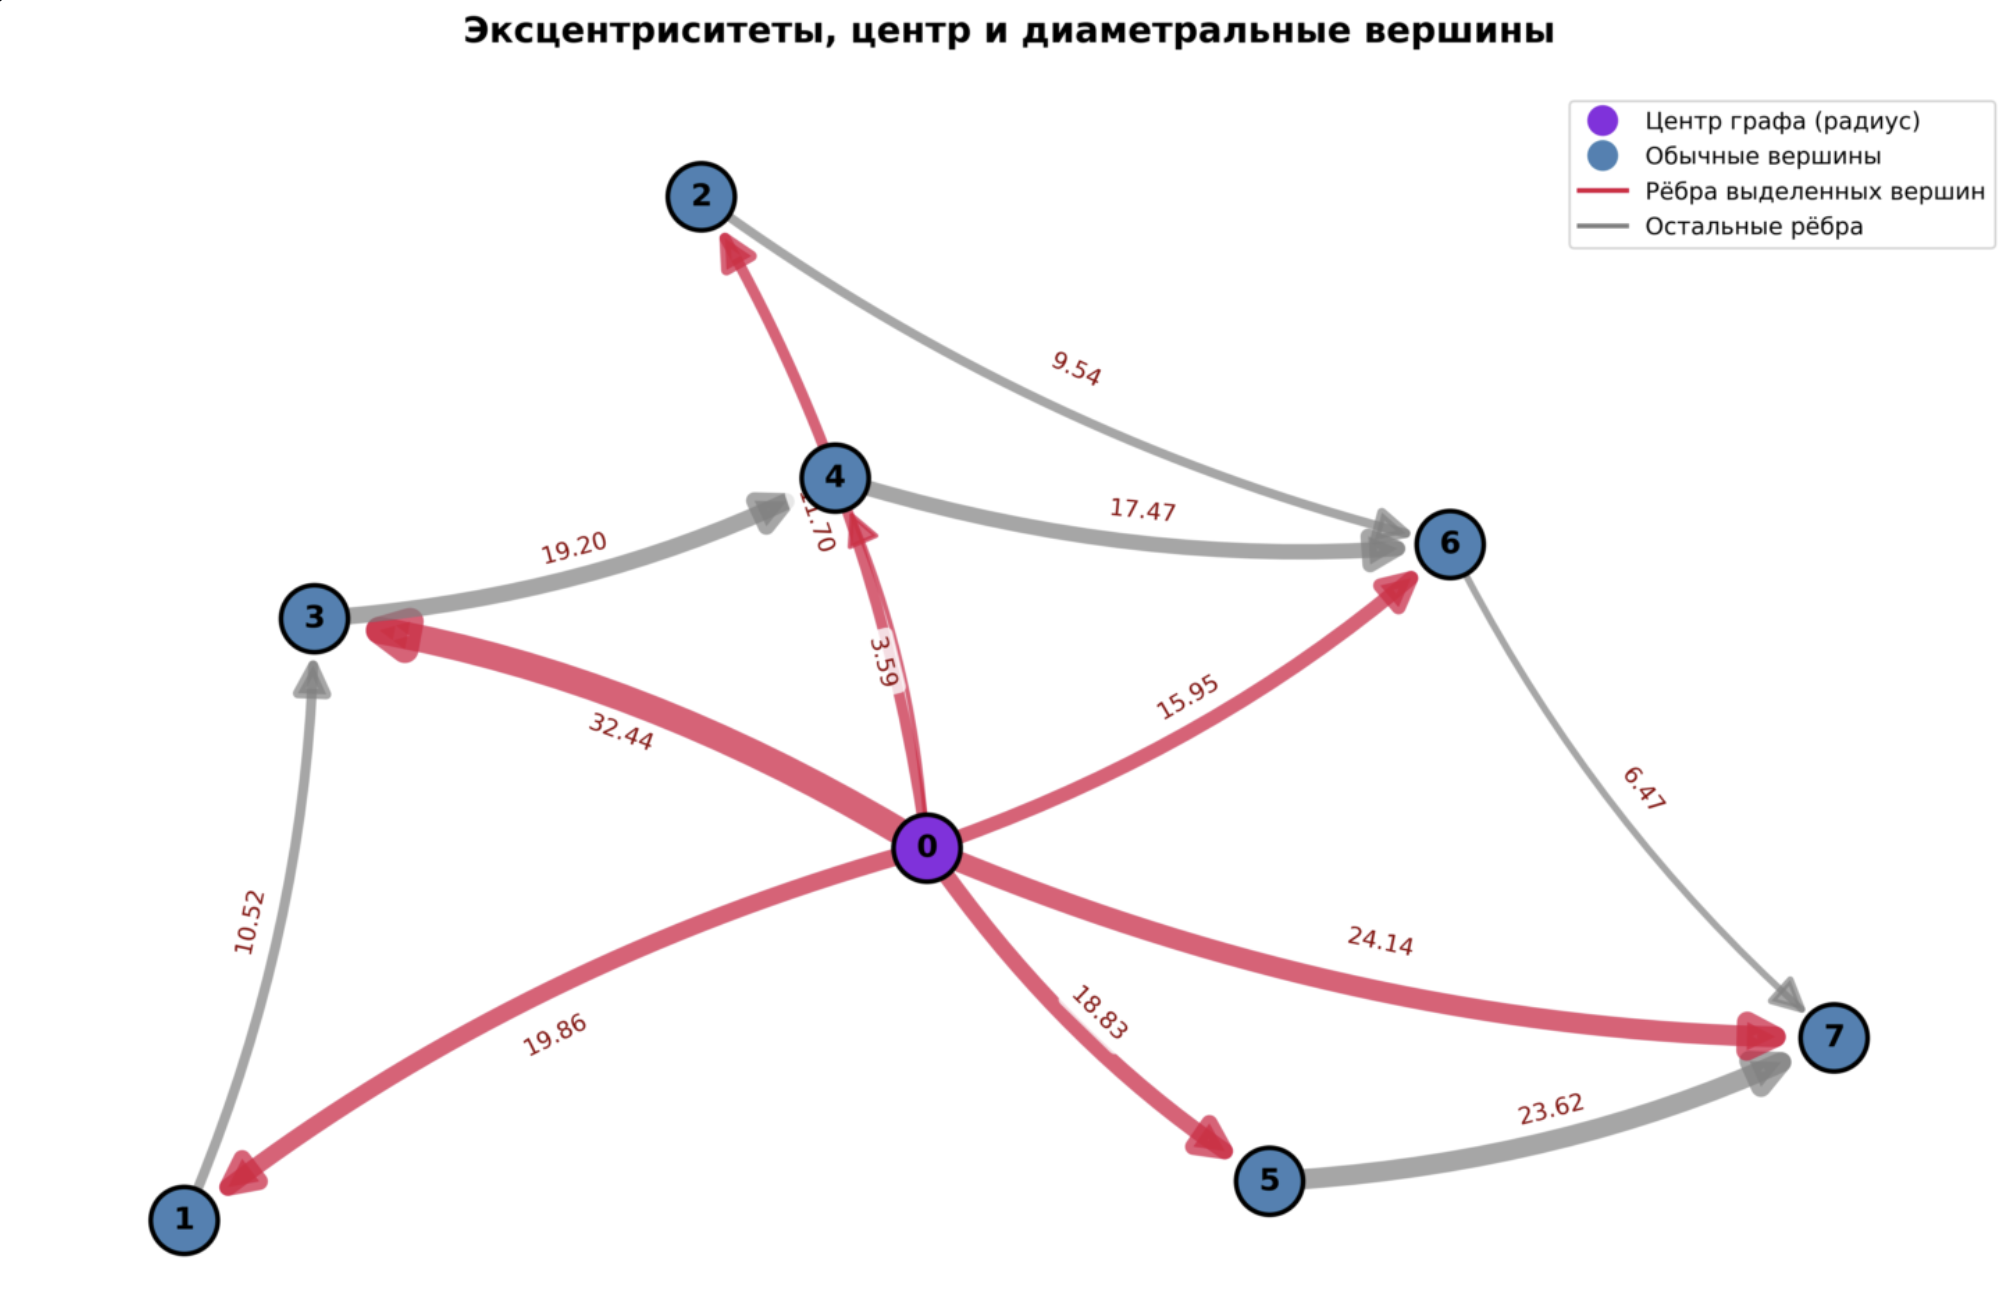
\includegraphics[width=1\linewidth]{images/lab1/exc.png}
    \caption{Орграф с выделением центра}
    \label{fig:ecc_graph}
\end{figure}

\begin{figure}[H]
    \centering
    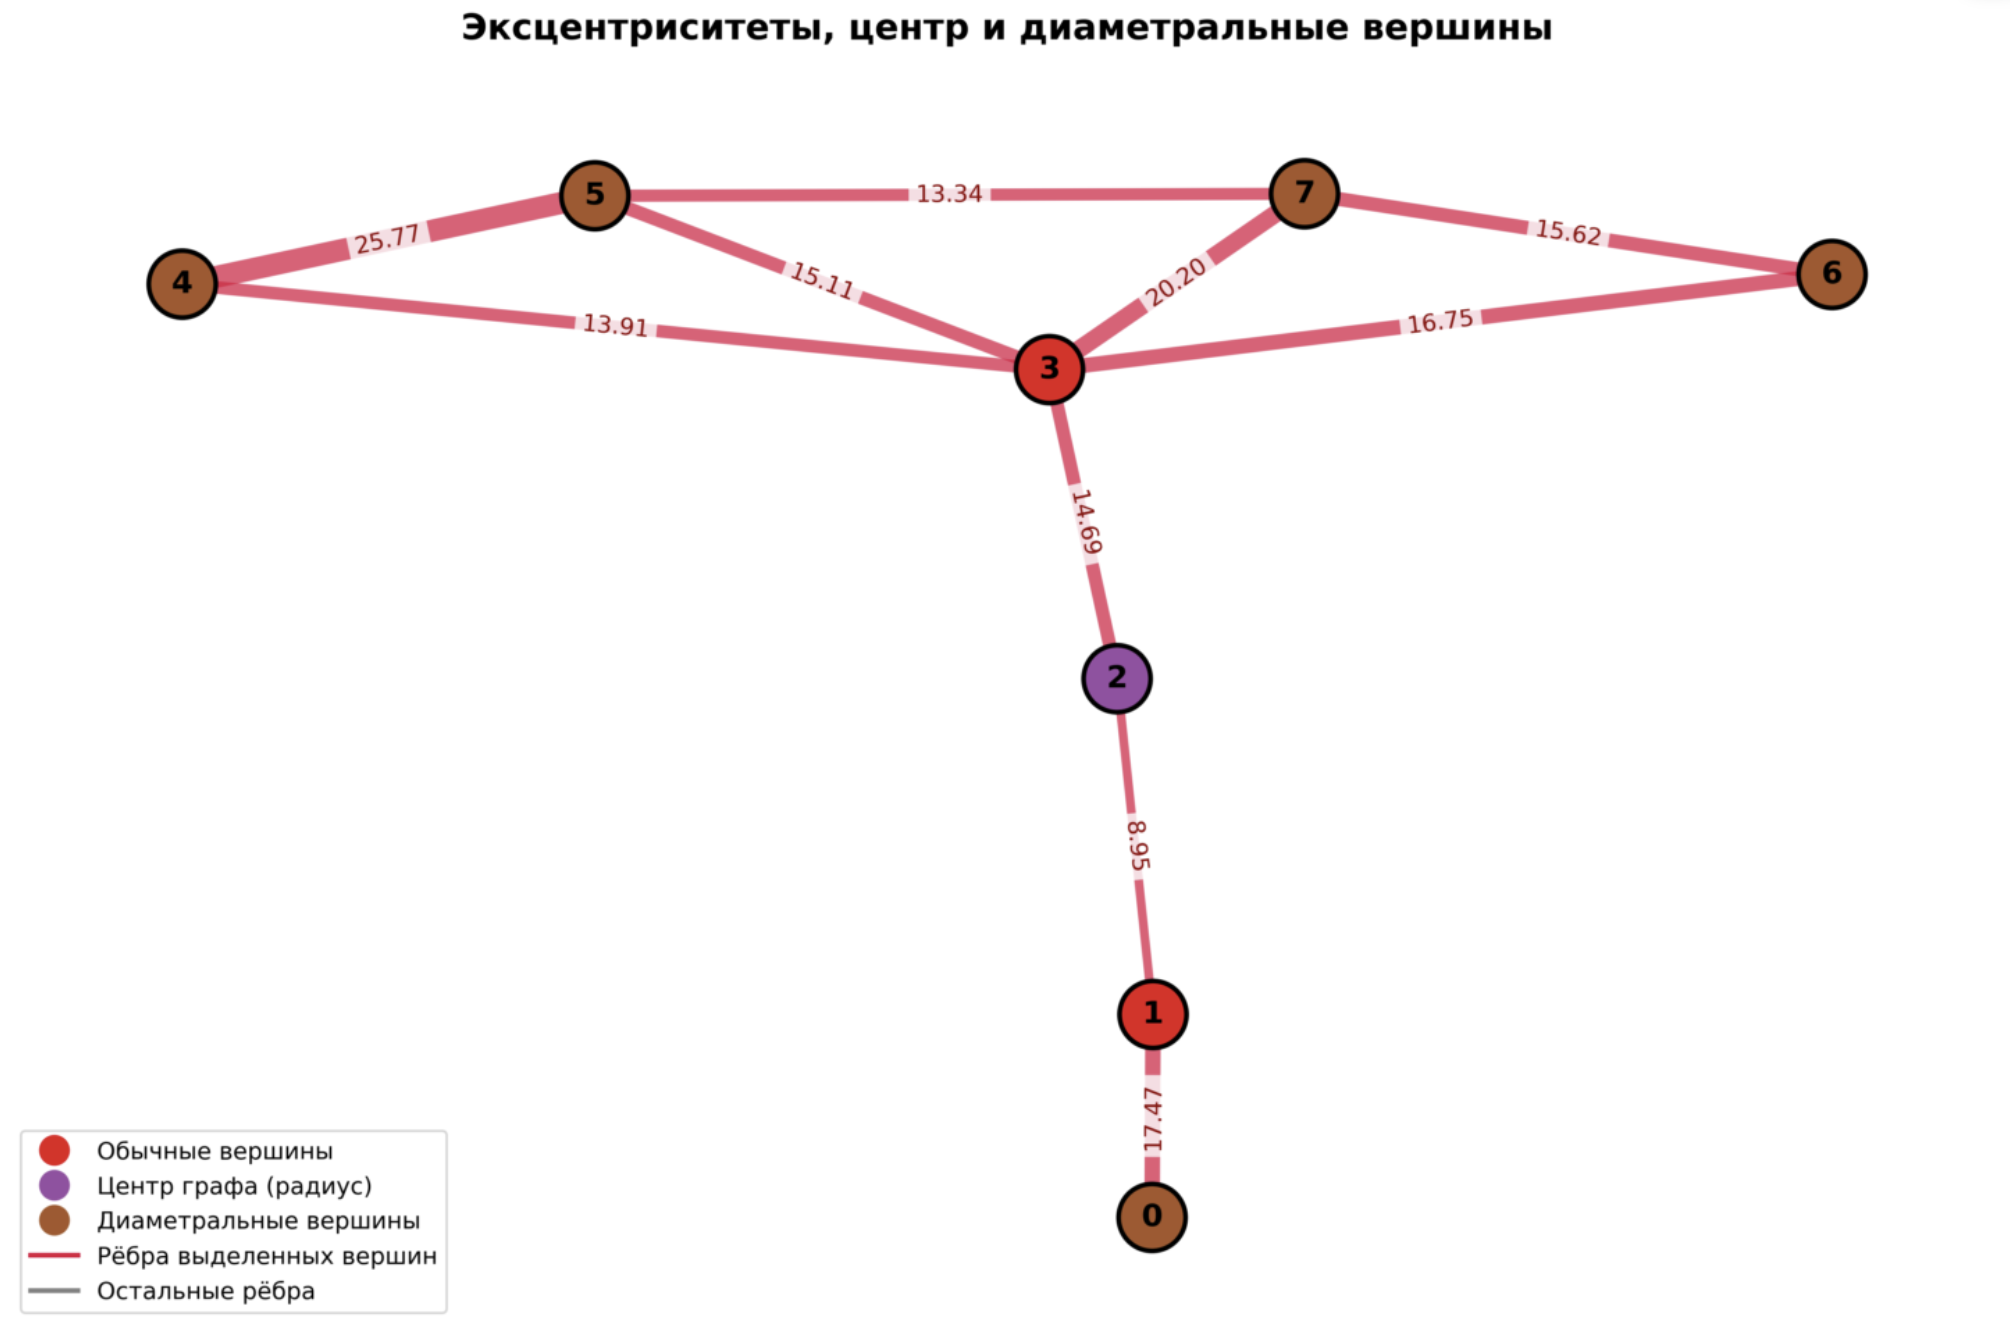
\includegraphics[width=1\linewidth]{images/lab1/exc1.png}
    \caption{Граф с выделением центра и диаметральных вершин}
    \label{fig:ecc_diameter}
\end{figure}

\begin{figure}[H]
    \centering
    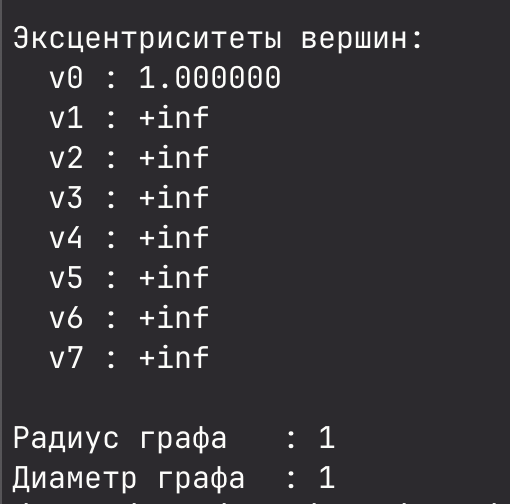
\includegraphics[width=0.4\linewidth]{images/lab1/exctxt.png}
    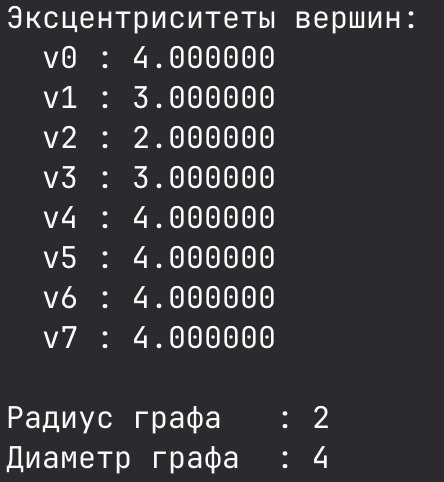
\includegraphics[width=0.362\linewidth]{images/lab1/exctxt1.png}
    \caption{Текстовый вывод метрик графа}
    \label{fig:ecc_text}
\end{figure}

В орграфе только вершина $v_0$ имеет конечный эксцентриситет; у остальных
вершин эксцентриситет равен $+\infty$. В неорграфе минимальное значение
эксцентриситета равно~$2$ (вершина $v_2$), максимальное~--- $4$
(вершины $v_0,\, v_4$--$v_7$).

% ─────────────────────────────────────────────────────────────────
\subsection{Лабораторная работа~2}
% ─────────────────────────────────────────────────────────────────

\subsubsection{Обход рёбер в ширину}

BFS запускается из вершины, заданной пользователем. Программа выводит
порядок посещения вершин, список рёбер дерева обхода и число итераций.
Рёбра дерева выделяются на визуализации (рис.~\ref{fig:bfs_tree}).

\begin{figure}[H]
    \centering
    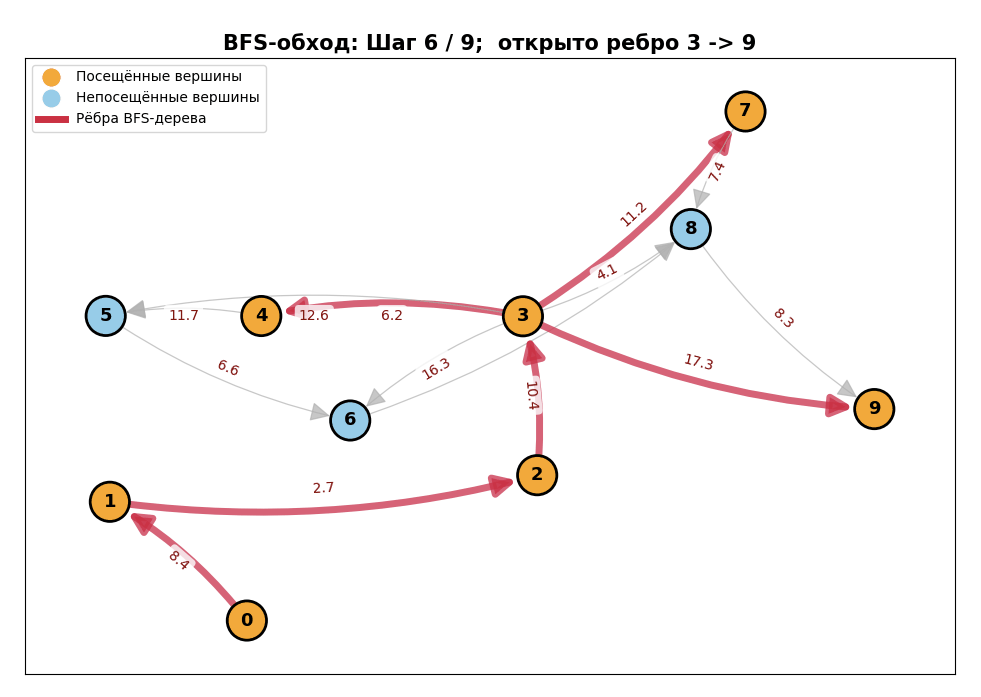
\includegraphics[width=0.82\linewidth]{images/lab2/bfs.png}
    \caption{Граф с выделенными рёбрами дерева BFS-обхода}
    \label{fig:bfs_tree}
\end{figure}

\subsubsection{Алгоритм Дейкстры}

Пользователь вводит начальную и конечную вершины. Программа выводит
вектор расстояний от источника до всех вершин, восстановленный путь
как последовательность вершин и число итераций. Результат показан на
рис.~\ref{fig:dijkstra}.

\begin{figure}[H]
    \centering
    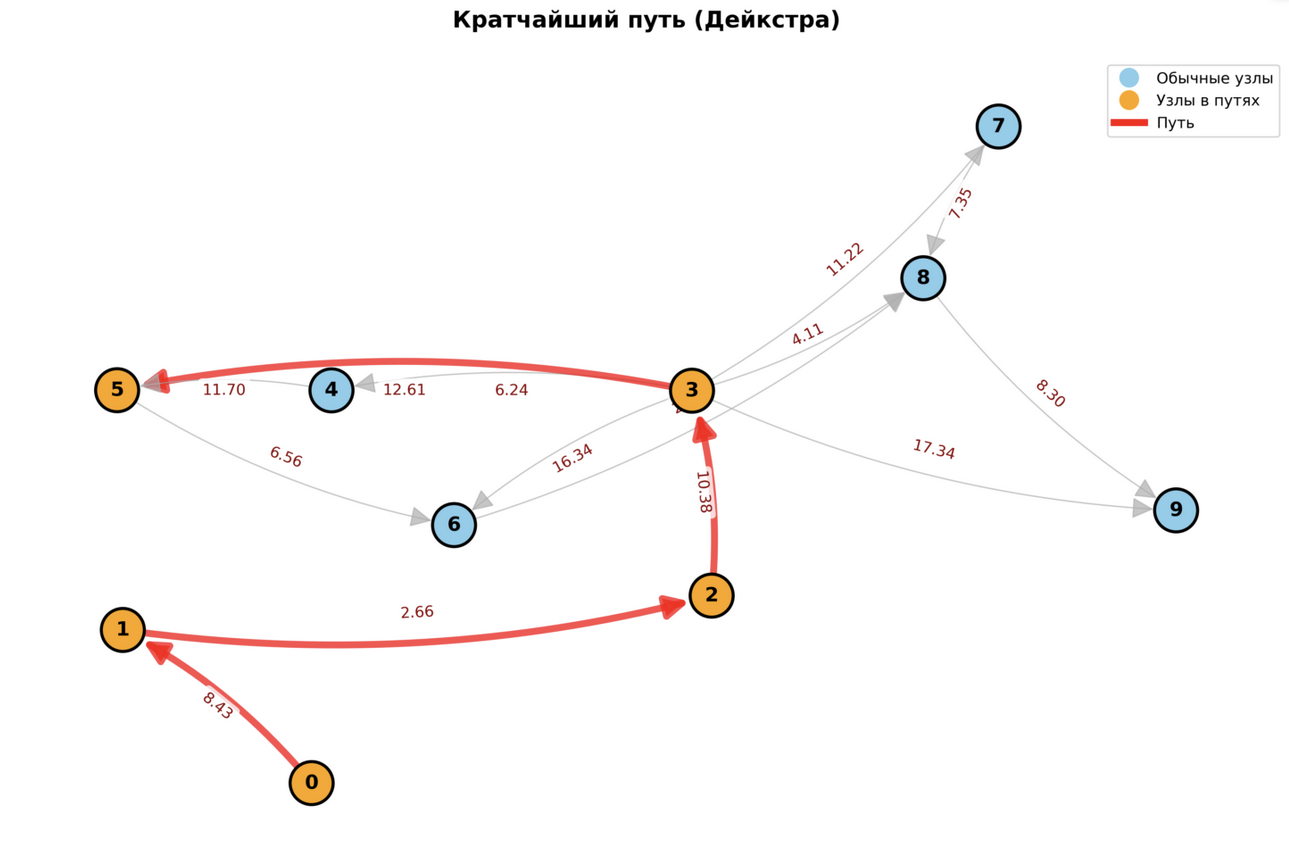
\includegraphics[width=0.9\linewidth]{images/lab2/deijkstra.png}
    \caption{Кратчайший путь по алгоритму Дейкстры}
    \label{fig:dijkstra}
\end{figure}

\subsubsection{Сравнение алгоритмов}

Оба алгоритма запускаются на одном графе с одной стартовой вершиной;
подсчитываются обращения как к рёбрам, так и к внутренним структурам
данных. Для теста был сгенерирован граф с~50 вершинами. Результат
представлен в виде гистограммы на рис.~\ref{fig:compare}.

\begin{figure}[H]
    \centering
    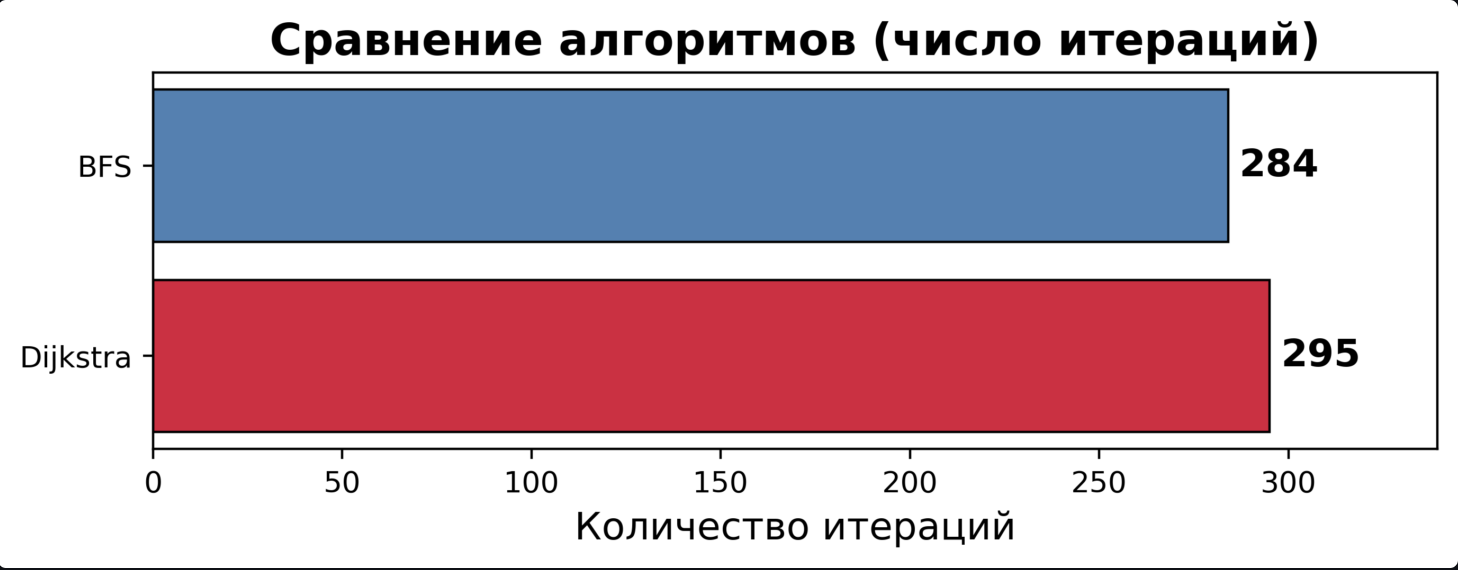
\includegraphics[width=0.7\linewidth]{images/lab2/compare.png}
    \caption{Сравнение числа итераций BFS и алгоритма Дейкстры}
    \label{fig:compare}
\end{figure}

% ─────────────────────────────────────────────────────────────────
\subsection{Лабораторная работа~3}
% ─────────────────────────────────────────────────────────────────

\subsubsection{Формирование сети потоков}

На основе ориентированного графа из предыдущих работ сформированы
матрицы пропускных способностей~$C$ и стоимостей дуг~$W$.
Визуализация приведена на рис.~\ref{fig:flow_network}
и~\ref{fig:lab3_matrices}.

\begin{figure}[H]
    \centering
    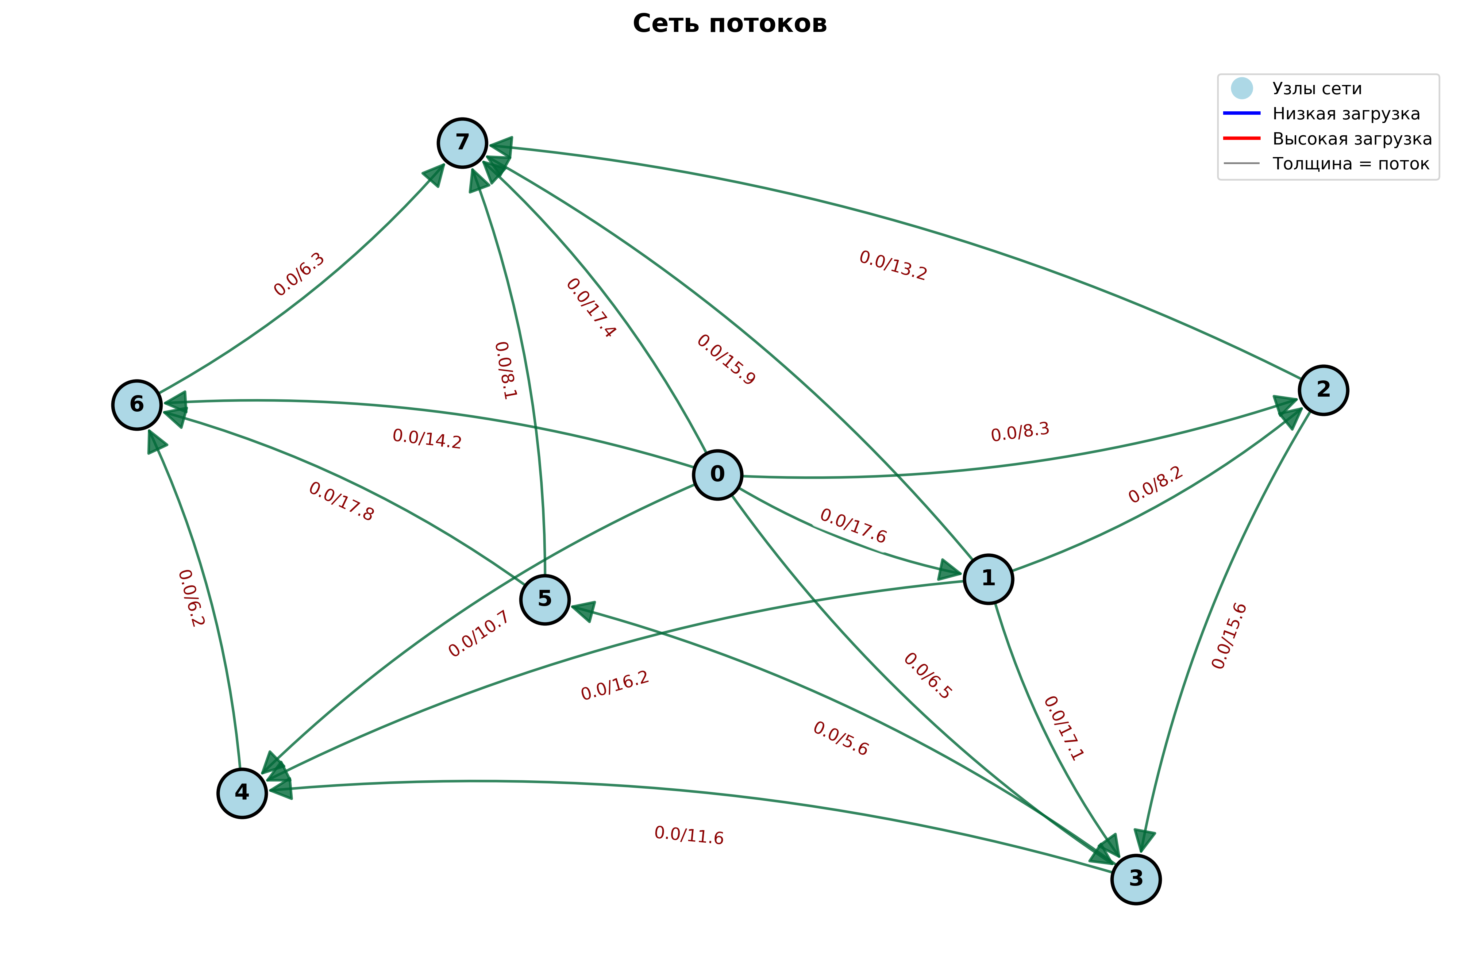
\includegraphics[width=0.85\linewidth]{images/lab3/flow net.png}
    \caption{Сеть потоков}
    \label{fig:flow_network}
\end{figure}

\begin{figure}[H]
    \centering
    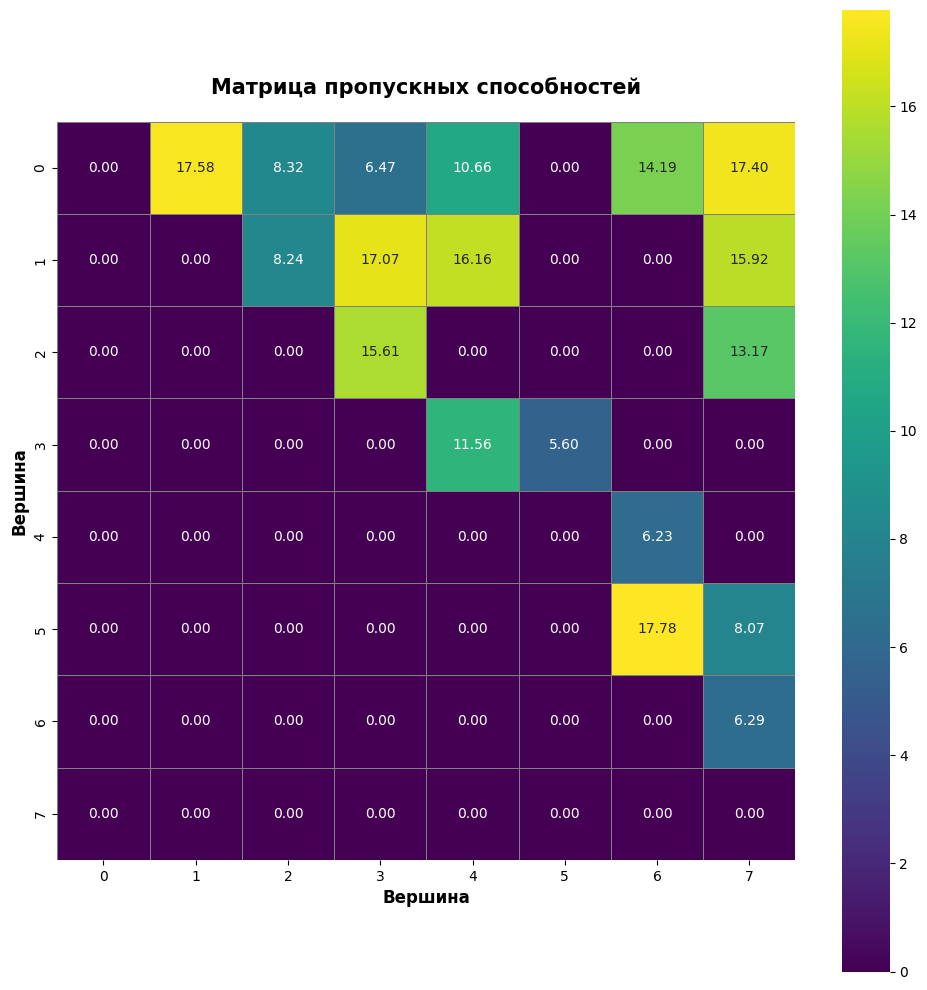
\includegraphics[width=0.48\linewidth]{images/lab3/capacities.png}%
    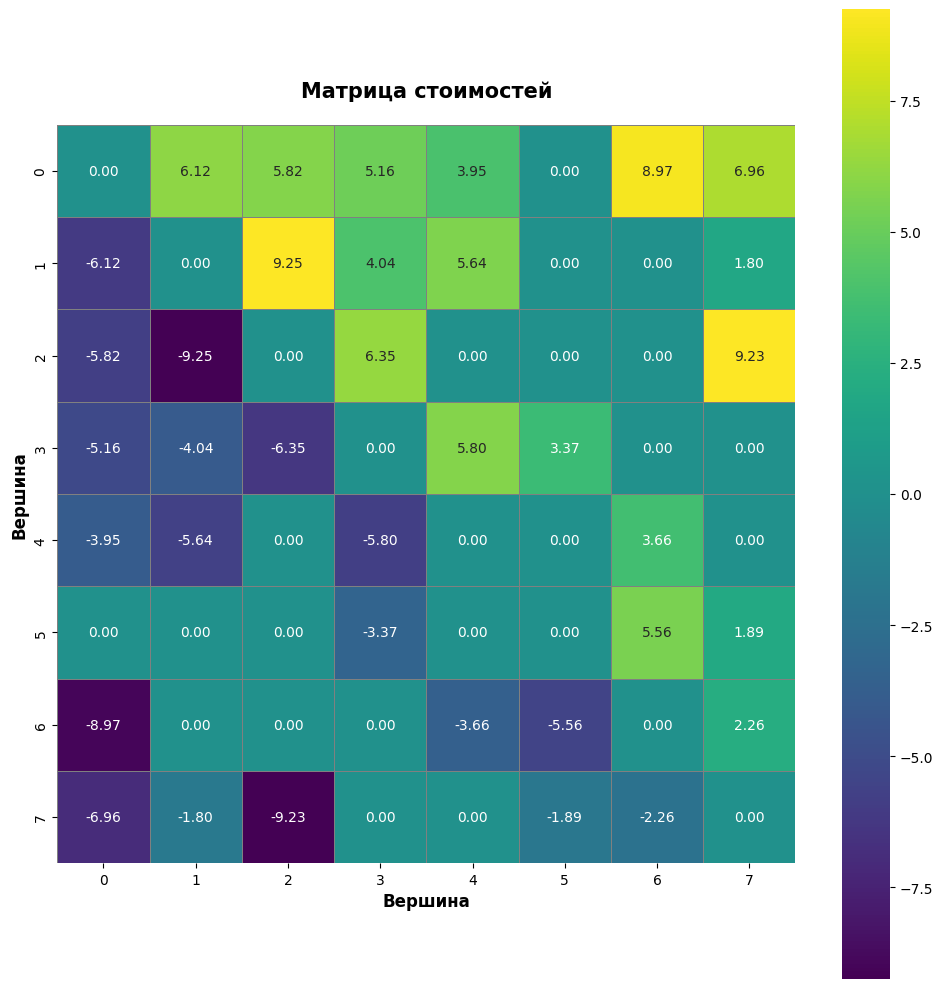
\includegraphics[width=0.48\linewidth]{images/lab3/costs.png}
    \caption{Матрица пропускных способностей (слева) и матрица стоимостей (справа)}
    \label{fig:lab3_matrices}
\end{figure}

\subsubsection{Максимальный поток}

Алгоритм Форда--Фалкерсона итеративно находит увеличивающие пути
в остаточной сети до их исчезновения. На рис.~\ref{fig:max_flow_graph}
показана финальная визуализация потока из вершины~$0$ в вершину~$7$.

\begin{figure}[H]
    \centering
    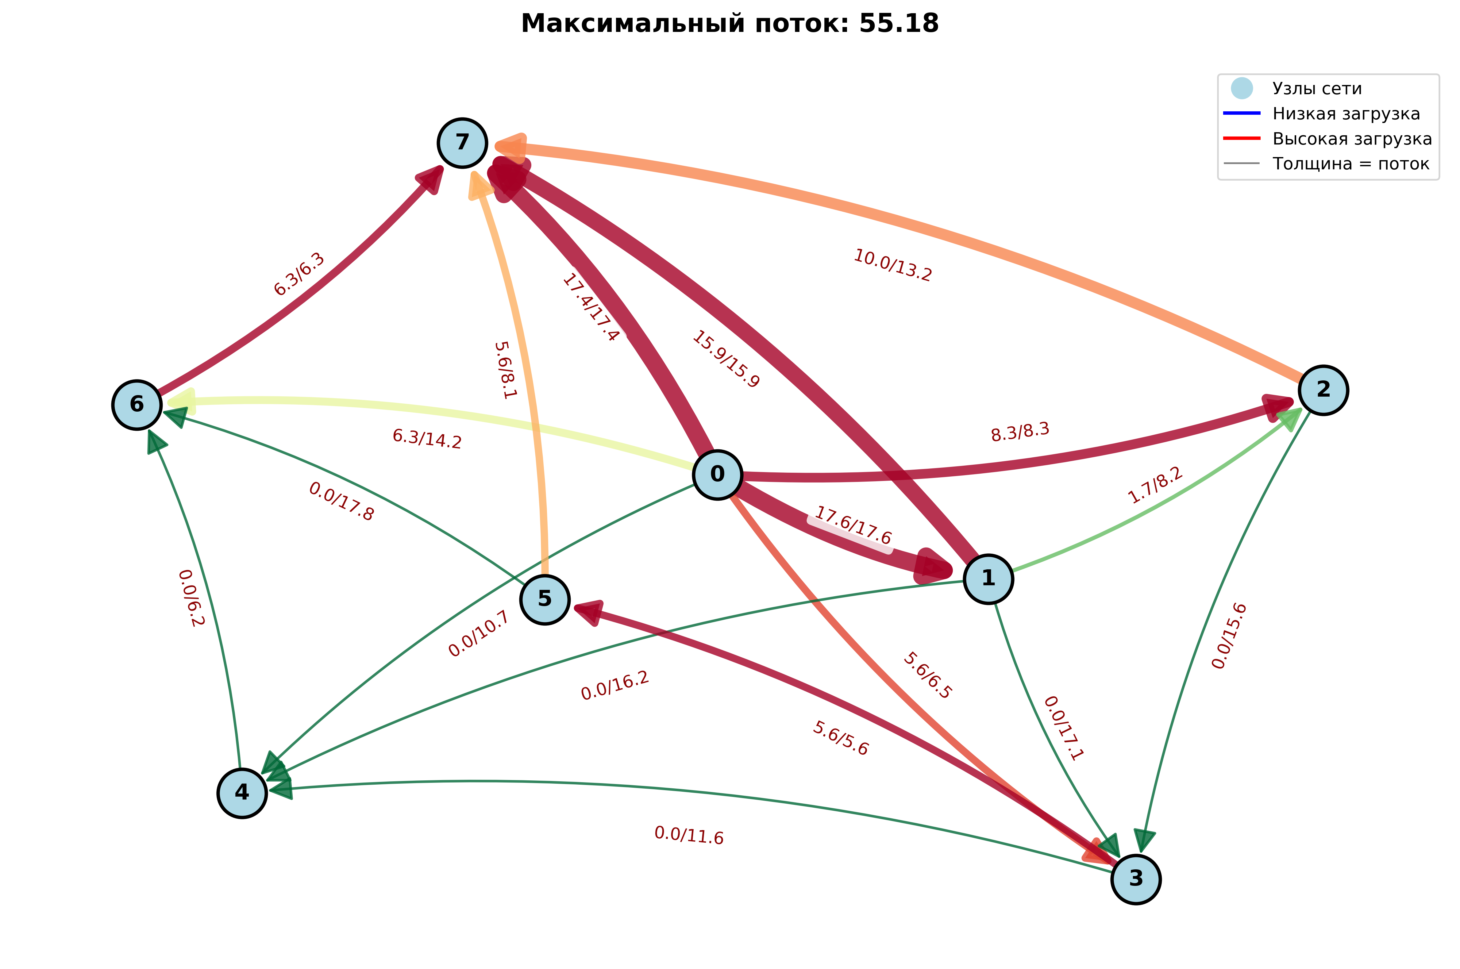
\includegraphics[width=1\linewidth]{images/lab3/max_flow.png}
    \caption{Распределение максимального потока в транспортной сети}
    \label{fig:max_flow_graph}
\end{figure}

\subsubsection{Поток минимальной стоимости}

Целевая величина потока $F = \lfloor \frac{2}{3} \cdot F_{\max} \rfloor$
достигается последовательным поиском кратчайших путей по стоимости
в остаточной сети алгоритмом Беллмана--Форда. Результат приведён на
рис.~\ref{fig:min_cost_res} и~\ref{fig:min_cost_console}.

\begin{figure}[H]
    \centering
    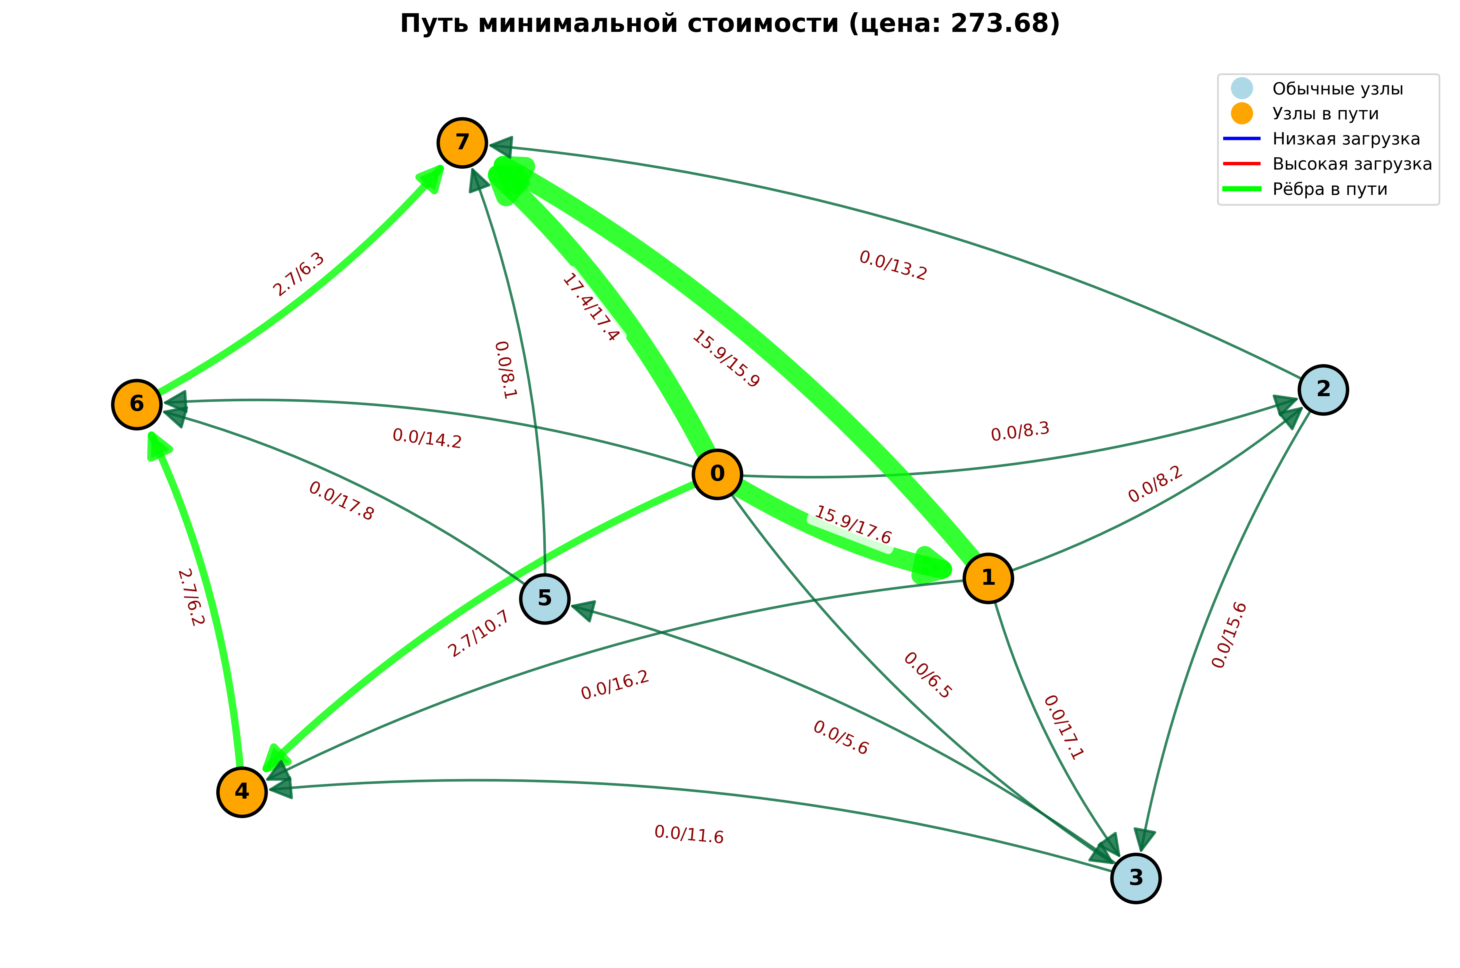
\includegraphics[width=1\linewidth]{images/lab3/min_cost.png}
    \caption{Поток минимальной стоимости величиной $\lfloor 2/3 \cdot F_{\max} \rfloor$}
    \label{fig:min_cost_res}
\end{figure}

\begin{figure}[H]
    \centering
    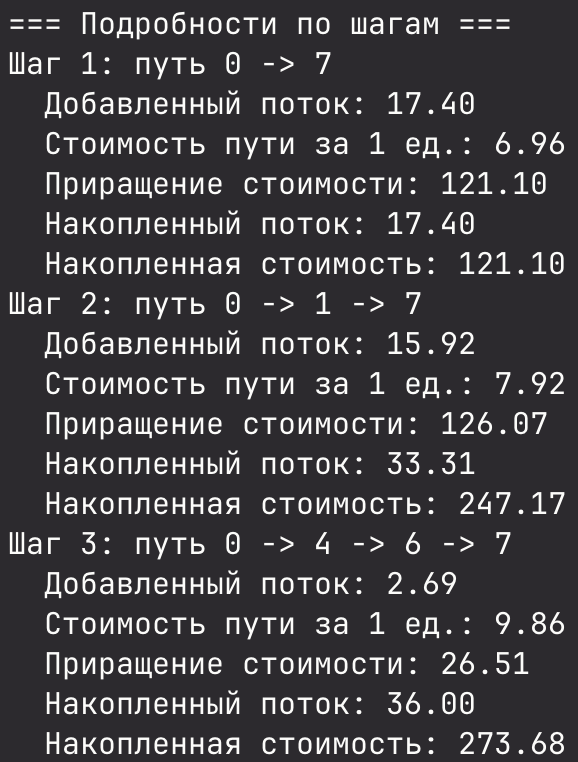
\includegraphics[width=0.42\linewidth]{images/lab3/min_cost_output.png}
    \caption{Консольный вывод: значение потока, суммарная стоимость, число итераций}
    \label{fig:min_cost_console}
\end{figure}

% ─────────────────────────────────────────────────────────────────
\subsection{Лабораторная работа~4}
% ─────────────────────────────────────────────────────────────────

Граф и матрица его смежности показаны на
рис.~\ref{fig:lab4_graph} и~\ref{fig:lab4_capacities}.

\begin{figure}[H]
    \centering
    
\includegraphics[width=0.9\linewidth]{images/lab4/graph.png}
    \caption{Исходный неориентированный взвешенный граф}
    \label{fig:lab4_graph}
\end{figure}

\begin{figure}[H]
    \centering
    
\includegraphics[width=0.6\linewidth]{images/lab4/capacities.png}
    \caption{Матрица смежности исходного графа}
    \label{fig:lab4_capacities}
\end{figure}

\subsubsection{Матричная теорема Кирхгофа}

Для данного графа число остовных деревьев
составило~$228$.

\subsubsection{Минимальный остов алгоритмом Борувки}

Программа строит МОД и выводит число рёбер и суммарный вес.
Визуализация приведена на рис.~\ref{fig:boruvka_mst}.

\begin{figure}[H]
    \centering
    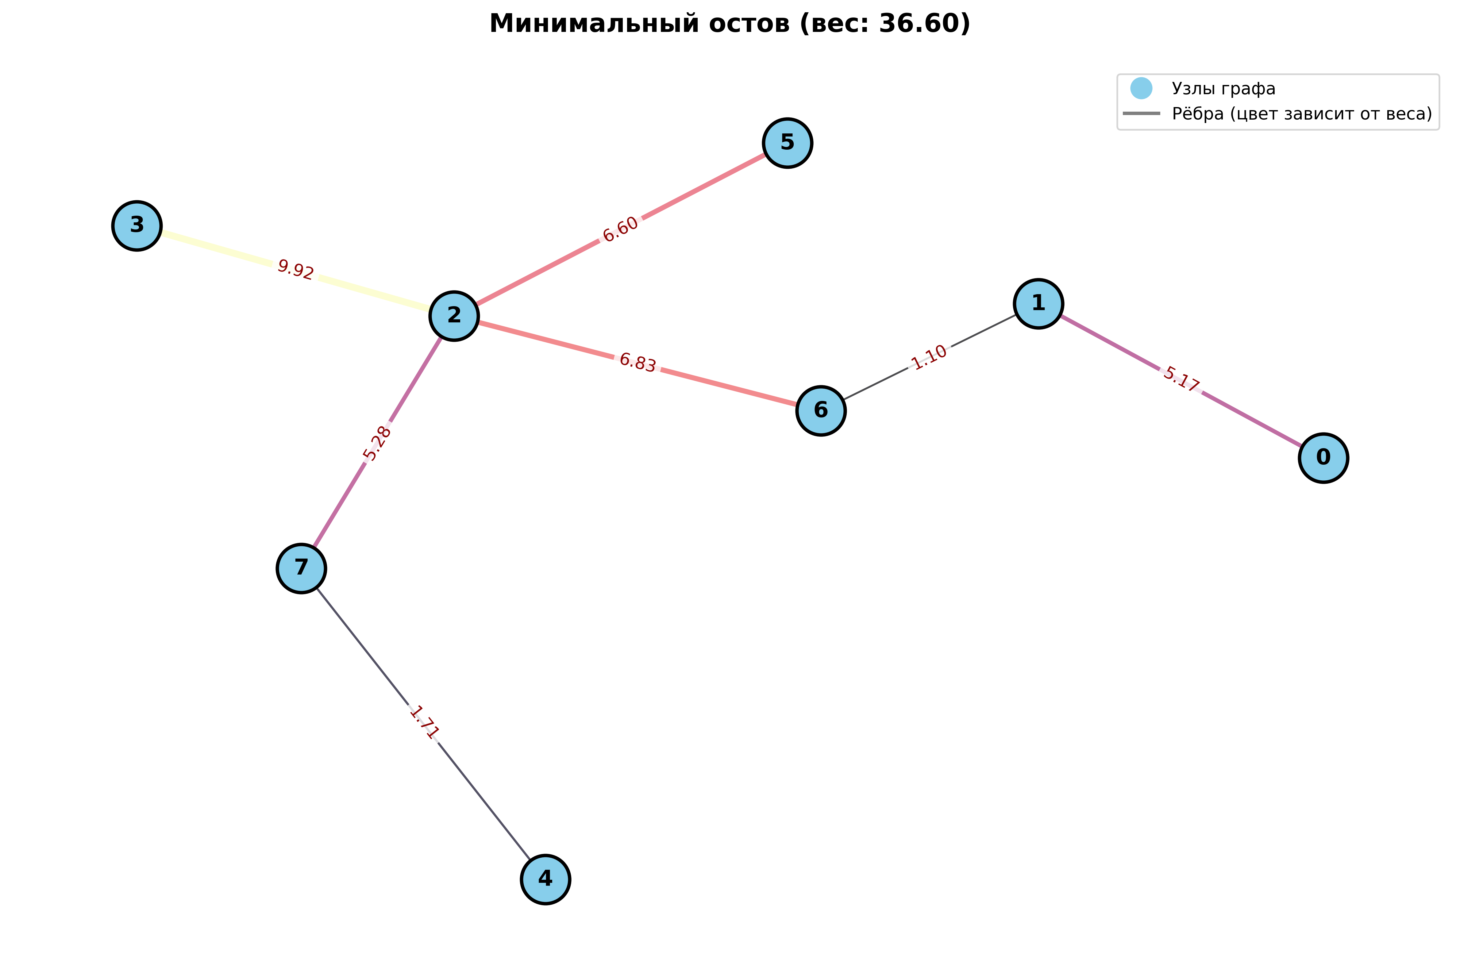
\includegraphics[width=1\linewidth]{images/lab4/boruvka_mst.png}
    \caption{Минимальное остовное дерево, построенное алгоритмом Борувки}
    \label{fig:boruvka_mst}
\end{figure}

\subsubsection{Кодирование и декодирование кода Прюфера}

Построенный МОД кодируется последовательностью Прюфера длины $n - 2$.
Для графа из~8 вершин последовательность имеет длину~6:

\[
    1\ 6\ 2\ 7\ 2\ 2.
\]
Декодированное дерево имеет тот же суммарный вес, что и исходный МОД,
что подтверждает корректность кодирования. Визуализация восстановленного
дерева приведена на рис.~\ref{fig:prufer_decoded}.

\begin{figure}[H]
    \centering
    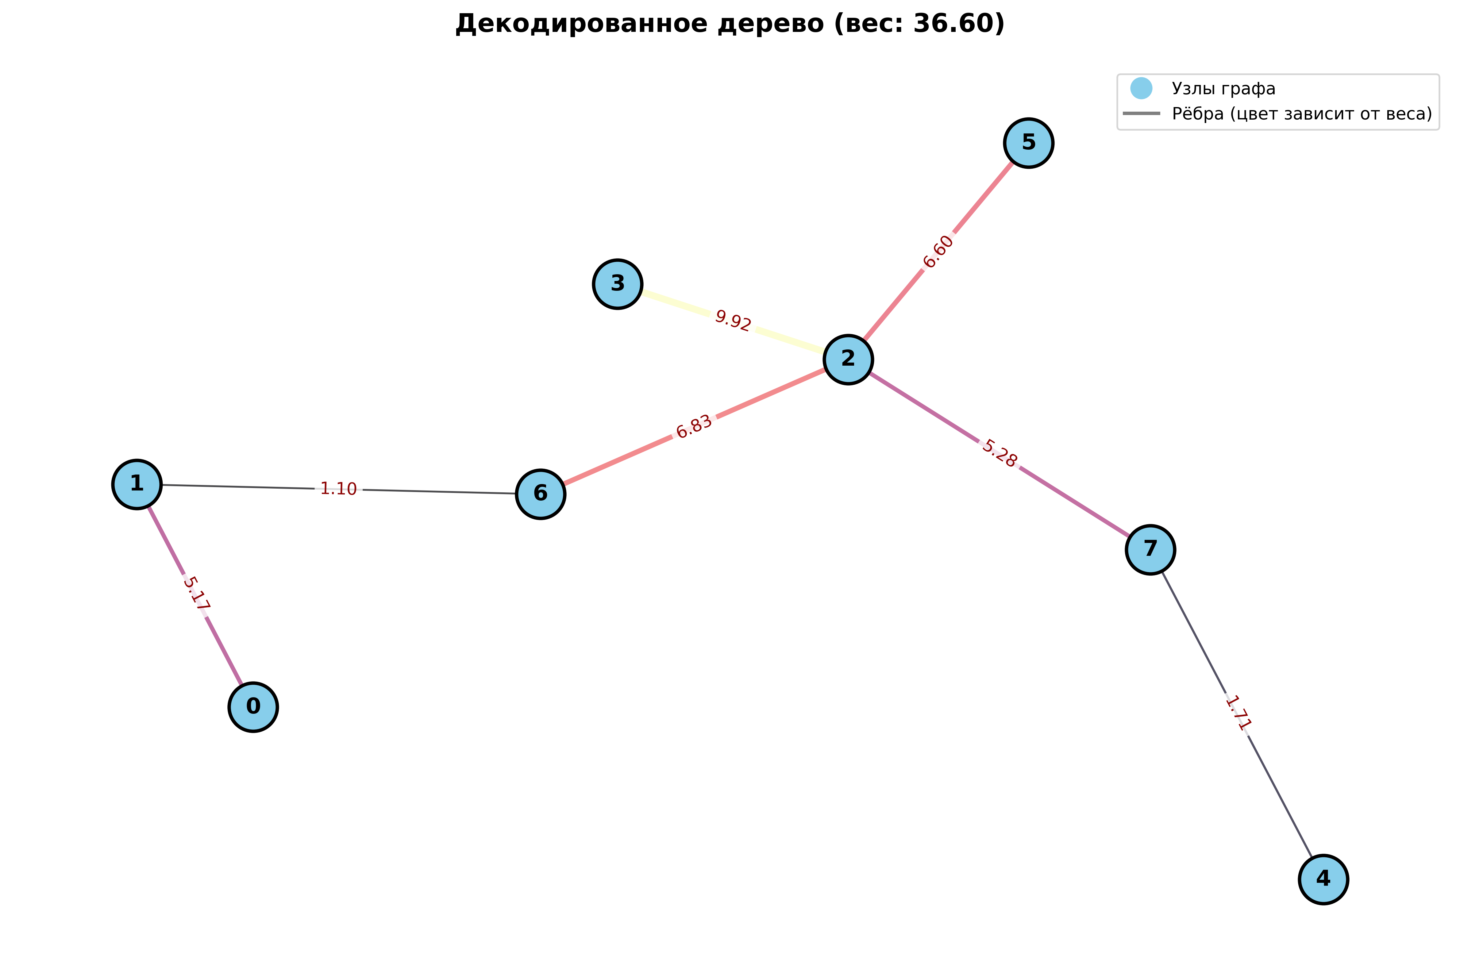
\includegraphics[width=0.85\linewidth]{images/lab4/prufer_decoded.png}
    \caption{Дерево, восстановленное из кода Прюфера}
    \label{fig:prufer_decoded}
\end{figure}

\subsubsection{Минимальная раскраска графа}

Пользователь выбирает граф для раскраски~--- исходный или МОД.
Программа перебором с возвратом находит хроматическое число $\chi(G)$
и выводит цвет каждой вершины. Визуализация с оптимальной раскраской
приведена на рис.~\ref{fig:coloring_graph}.

\begin{figure}[H]
    \centering
    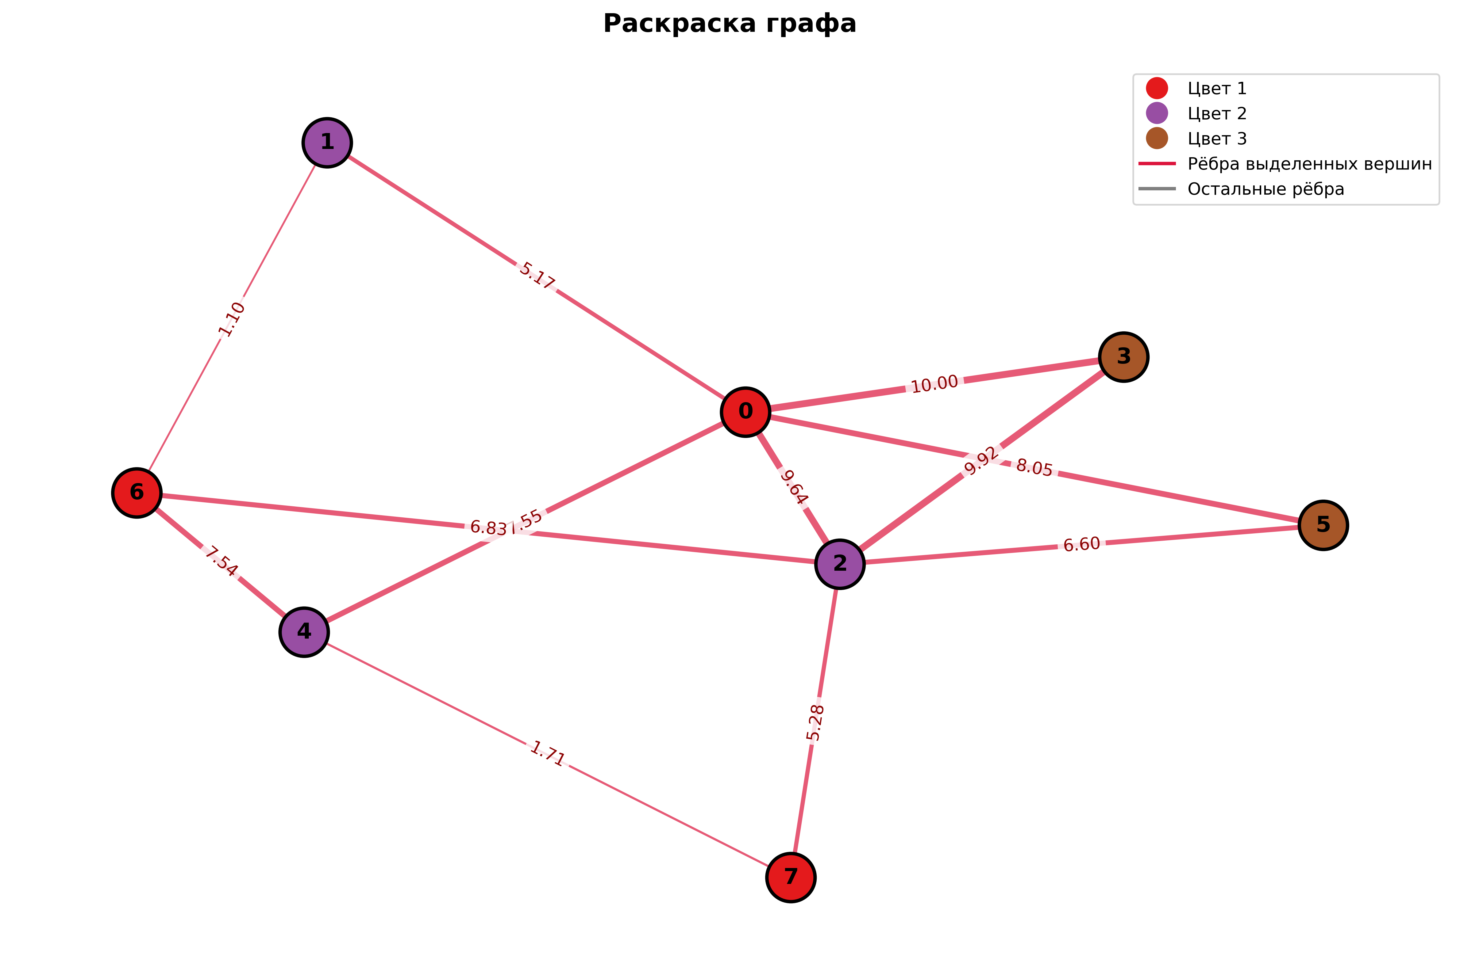
\includegraphics[width=0.85\linewidth]{images/lab4/coloring_graph.png}
    \caption{Граф с минимальной раскраской вершин}
    \label{fig:coloring_graph}
\end{figure}

% ─────────────────────────────────────────────────────────────────
\subsection{Лабораторная работа~5}
% ─────────────────────────────────────────────────────────────────

\subsubsection{Проверка эйлеровости и построение эйлерова цикла}

Достроенный граф до эйлерова с визуализированным эйлеровым циклом на нем показан на
рис.~\ref{fig:euler_graph} и~\ref{fig:euler_output}.

\begin{figure}[H]
    \centering
    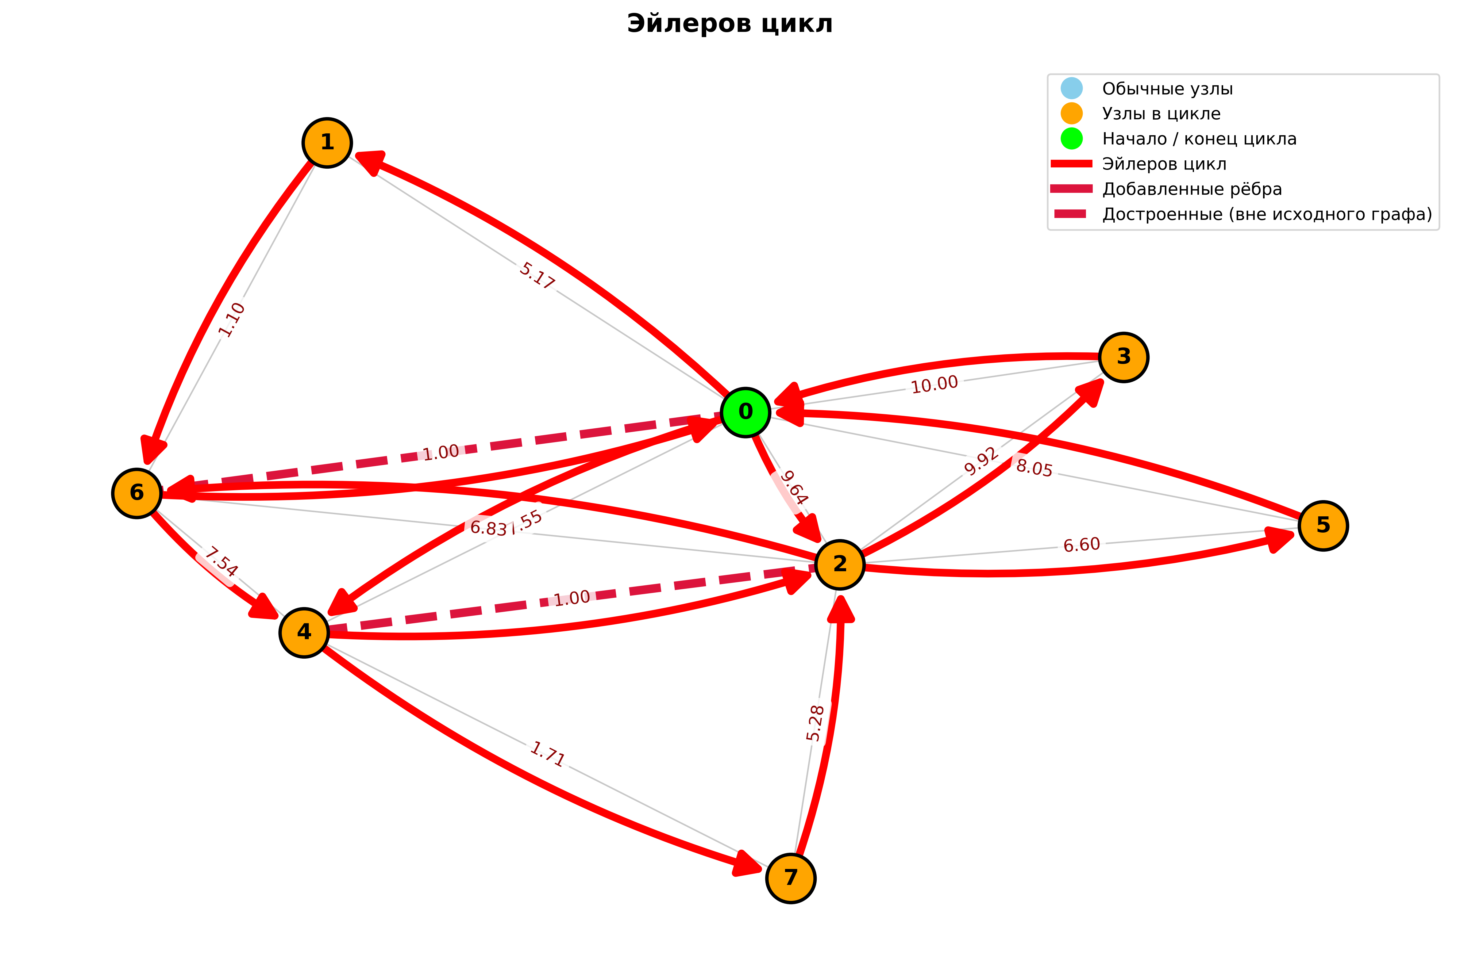
\includegraphics[width=1\linewidth]{images/lab5/euler_graph.png}
    \caption{Граф с выделенным эйлеровым циклом; добавленные рёбра отмечены отдельным цветом}
    \label{fig:euler_graph}
\end{figure}

\begin{figure}[H]
    \centering
    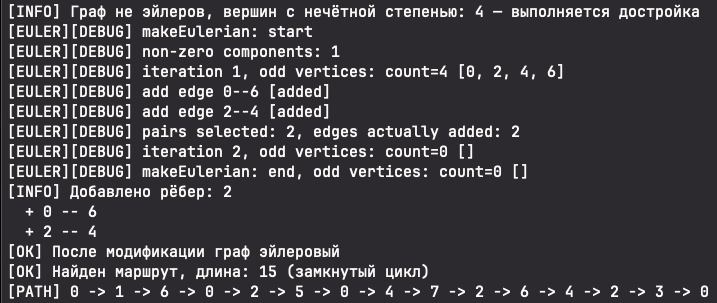
\includegraphics[width=0.6\linewidth]{images/lab5/euler_output.png}
    \caption{Консольный вывод: результат проверки, добавленные рёбра и маршрут}
    \label{fig:euler_output}
\end{figure}

\subsubsection{Фундаментальная система разрезов}

Программа строит МОД алгоритмом Борувки и вычисляет фундаментальный разрез для каждого ребра остова. Визуализация МОД приведена на рис.~\ref{fig:lab5_mst}; визуальный вывод ФСР~--- на рис.~\ref{fig:cuts_output}.

\begin{figure}[H]
    \centering
    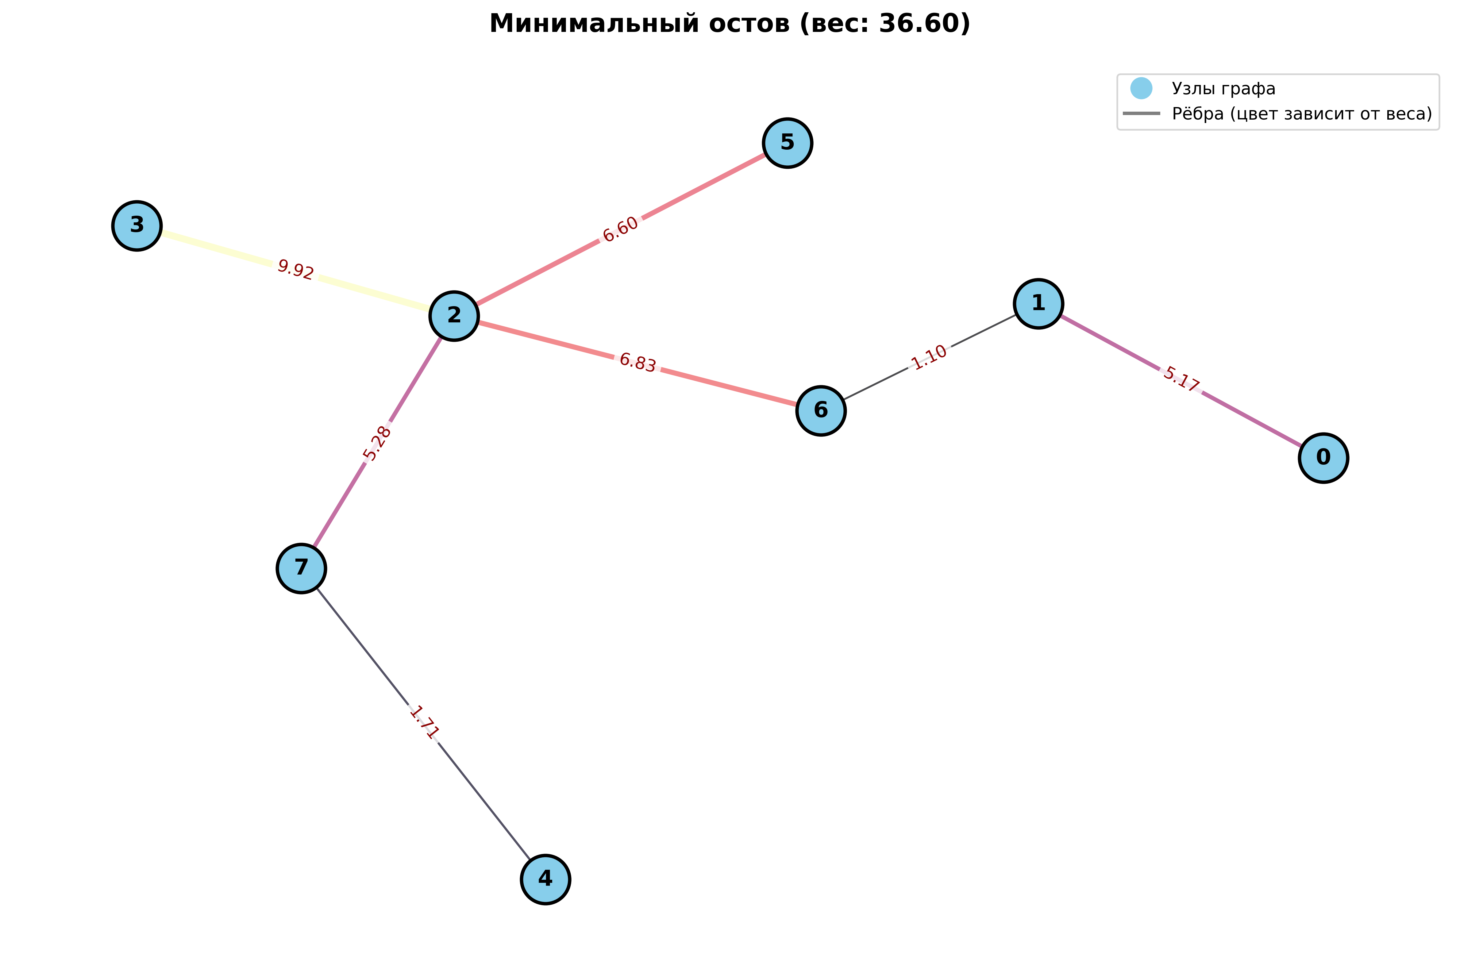
\includegraphics[width=1\linewidth]{images/lab5/mst.png}
    \caption{Минимальный остов, построенный алгоритмом Борувки}
    \label{fig:lab5_mst}
\end{figure}

\begin{figure}[H]
    \centering
    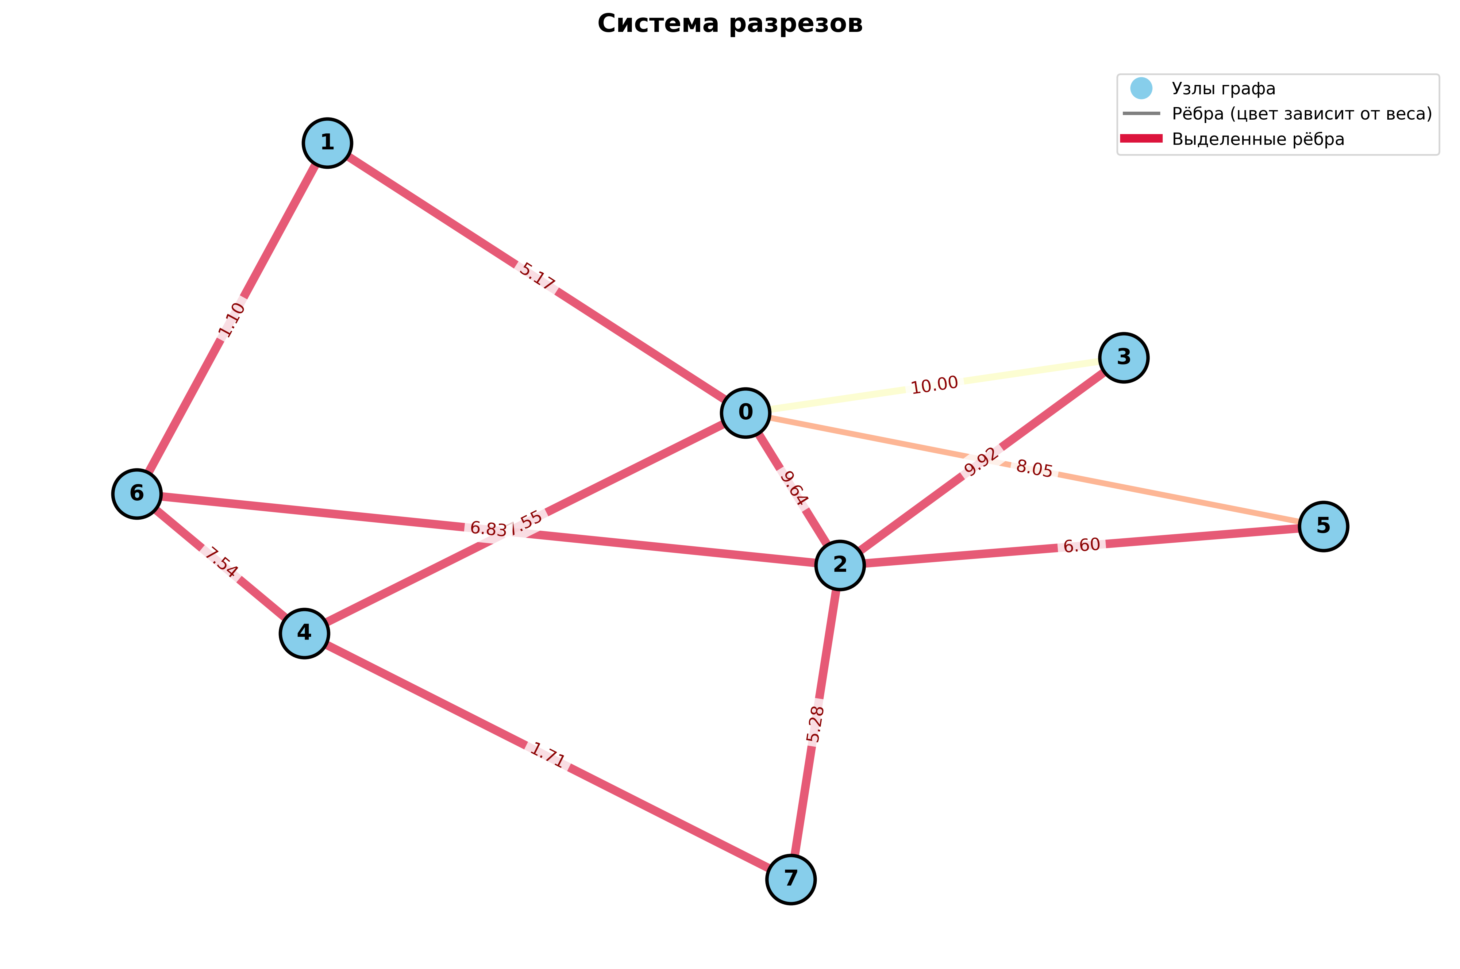
\includegraphics[width=1\linewidth]{images/lab5/cuts_graph.png}
    \caption{Граф: фундаментальная система разрезов}
    \label{fig:cuts_output}
\end{figure}

Фундаментальная система разрезов:
\begin{enumerate}
    \item[0)] Удалено $(2, 6)$ $\Rightarrow$ $A = \{2, 3, 4, 5, 7\}$, $B = \{0, 1, 6\}$. \\ Разрез: $\{(0, 2), (0, 3), (0, 4), (0, 5), (2, 6), (4, 6)\}$.
    \item[1)] Удалено $(2, 7)$ $\Rightarrow$ $A = \{0, 1, 2, 3, 5, 6\}$, $B = \{4, 7\}$. \\ Разрез: $\{(0, 4), (2, 7), (4, 6)\}$.
    \item[2)] Удалено $(2, 3)$ $\Rightarrow$ $A = \{0, 1, 2, 4, 5, 6, 7\}$, $B = \{3\}$. \\ Разрез: $\{(0, 3), (2, 3)\}$.
    \item[3)] Удалено $(2, 5)$ $\Rightarrow$ $A = \{0, 1, 2, 3, 4, 6, 7\}$, $B = \{5\}$. \\ Разрез: $\{(0, 5), (2, 5)\}$.
    \item[4)] Удалено $(1, 6)$ $\Rightarrow$ $A = \{0, 1\}$, $B = \{2, 3, 4, 5, 6, 7\}$. \\ Разрез: $\{(0, 2), (0, 3), (0, 4), (0, 5), (1, 6)\}$.
    \item[5)] Удалено $(0, 1)$ $\Rightarrow$ $A = \{0\}$, $B = \{1, 2, 3, 4, 5, 6, 7\}$. \\ Разрез: $\{(0, 1), (0, 2), (0, 3), (0, 4), (0, 5)\}$.
    \item[6)] Удалено $(4, 7)$ $\Rightarrow$ $A = \{4\}$, $B = \{0, 1, 2, 3, 5, 6, 7\}$. \\ Разрез: $\{(0, 4), (4, 6), (4, 7)\}$.
\end{enumerate}

Симметрическая разность по всем разрезам: \\
$\{(0, 1), (0, 2), (0, 4), (1, 6), (2, 3), (2, 5), (2, 6), (2, 7), (4, 6), (4, 7)\}$. \\
При передаче пустого множества алгоритм возвращает исходную ФСР.

\subsubsection{Симметрическая разность подмножества разрезов}

Программа позволяет выбрать произвольное подмножество базовых разрезов (для примера выбраны разрезы $0, 2$ и $4$) и вычисляет их симметрическую разность. Результирующий разрез выводится в консоль и выделяется цветом на графе (рис.~\ref{fig:symdiff_graph} и~\ref{fig:symdiff_output}).

\begin{figure}[H]
    \centering
    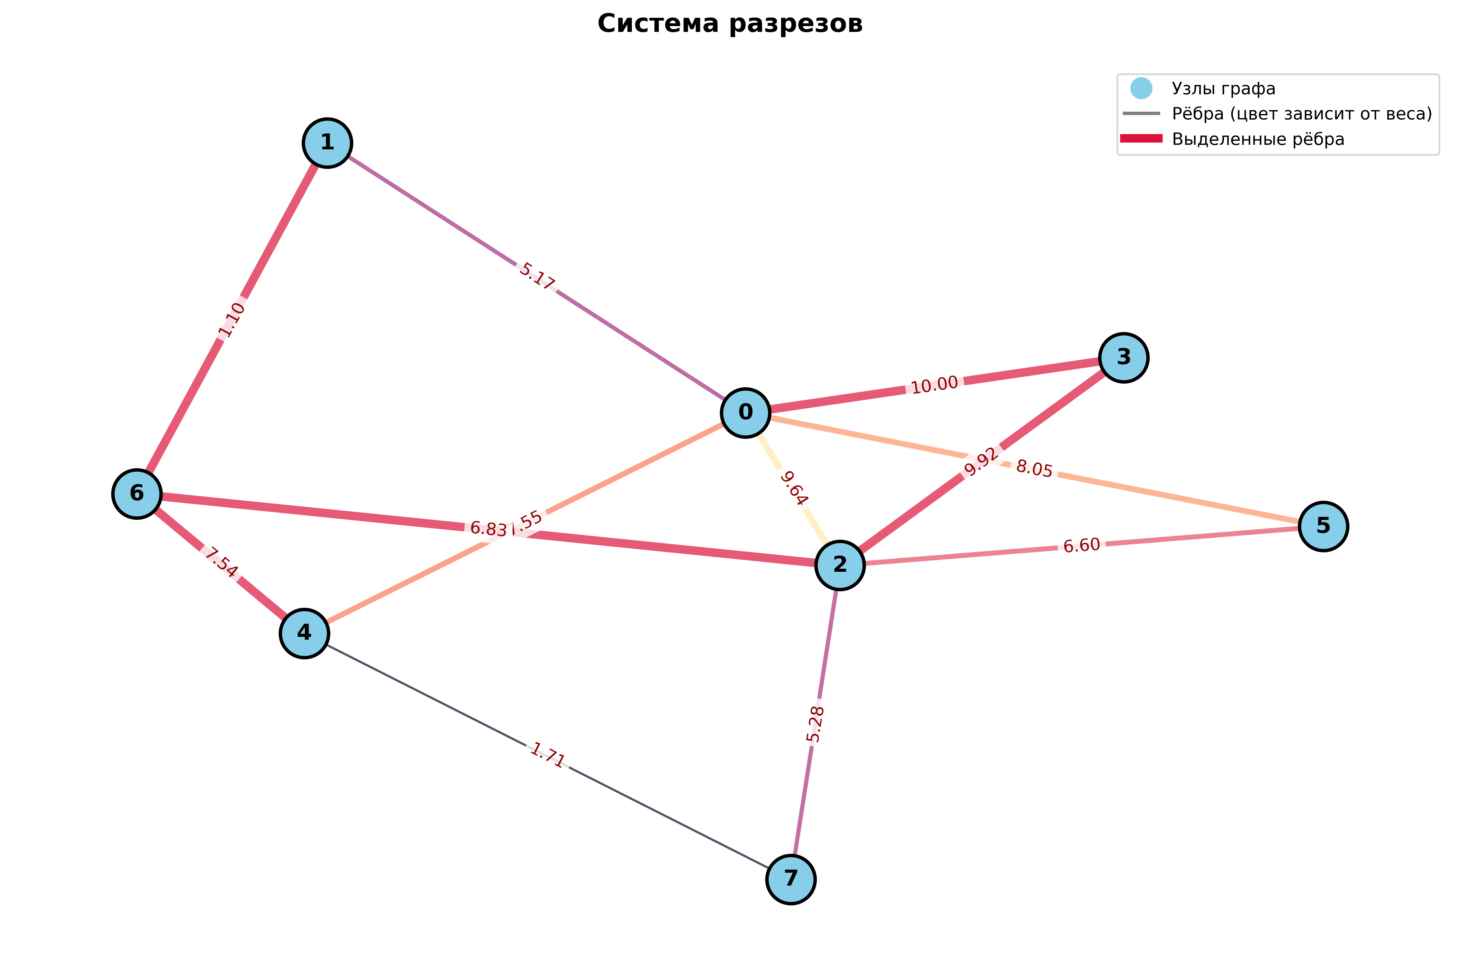
\includegraphics[width=1\linewidth]{images/lab5/symdiff_graph.png}
    \caption{Граф с выделенными рёбрами симметрической разности}
    \label{fig:symdiff_graph}
\end{figure}

\begin{figure}[H]
    \centering
    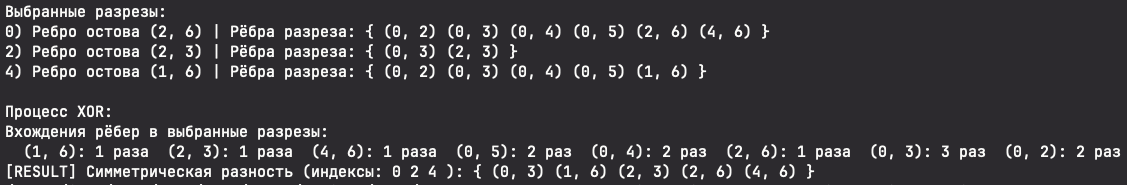
\includegraphics[width=1\linewidth]{images/lab5/symdiff_output.png}
    \caption{Консольный вывод: вхождения рёбер и результирующий разрез}
    \label{fig:symdiff_output}
\end{figure}
